
\chapter{Manifolds}

\section{Manifolds}

\begin{definition}[\emph{charts}]
  Let \(M\) be a topological space, a \emph{chart} on \(M\) is a tuple \((\varphi,U,V)\) where \begin{itemize}
    \item \(\varphi:U\to V\) is a homeomorphism, and
    \item \(U\) is an open subset of \(M\), and
    \item \(V\) is an open subset of \(\R^n\) for some \(n\).
  \end{itemize}
  % We say \((\f,U,V)\) is \emph{centered at \(p\)} if \(p\in U\) and \(\f(p) = 0\).
\end{definition}

\begin{center}
  \begin{tikzpicture}[
    manifold/.style={
        draw=black,
        fill=gray!10,
        line width=1pt
    },
    chart/.style={
        draw=blue!75!black,
        fill=blue!30,
        fill opacity=0.7,
        draw opacity=1,
        line width=1pt
    },
    chartarrow/.style={
        ->,
        blue!75!black,
        line width=0.5pt
    },
    axis/.style={
        -Stealth,
        black,
        line width=1pt
    }
]

% ------------------------------------------------
% Curved ambient sheet M
% ------------------------------------------------

\draw[manifold]
    (-5.30,-1.15)
    .. controls (-4.20,-1.65) and (-2.70,-1.10) ..
    (-1.20,-1.38)
    .. controls (-0.78,-0.72) and (-0.75,0.72) ..
    (-1.15,1.48)
    .. controls (-2.30,1.78) and (-3.75,1.25) ..
    (-5.05,1.55)
    .. controls (-5.42,0.83) and (-5.50,-0.35) ..
    cycle;

\node[black] at (-0.7,-1.2) {\(M\)};

% ------------------------------------------------
% Smaller curvilinear chart domain U
%
% The upper and lower edges follow the local
% curvature of the corresponding boundaries of M.
% The side edges bend toward the right, following
% the curvature of the right-hand boundary of M.
% ------------------------------------------------

\draw[chart]
    (-2.95,-0.38)
    .. controls (-2.58,-0.35) and (-2.02,-0.29) ..
    (-1.60,-0.38)
    .. controls (-1.5,-0.22) and (-1.5,0.25) ..
    (-1.58,0.60)
    .. controls (-2.00,0.75) and (-2.53,0.65) ..
    (-2.92,0.6)
    .. controls (-3.02,0.30) and (-3.04,-0.10) ..
    cycle;

\node[blue!75!black] at (-2.27,0.15) {\(U\)};

% ------------------------------------------------
% Coordinate axes for R^2
% ------------------------------------------------

\coordinate (O) at (1.85,-1.25);

\draw[axis]
    (O) -- ++(3.30,0)
    node[right] {\(\R^2\)};

\draw[axis]
    (O) -- ++(0,2.75);

% ------------------------------------------------
% Smaller rectangular coordinate image V
% ------------------------------------------------

\draw[chart]
    (2.45,-0.52)
    rectangle
    (4.30,0.72);

\node[blue!75!black]
    at (3.375,0.10) {\(V\)};

% ------------------------------------------------
% Straight chart map
% ------------------------------------------------

\draw[chartarrow]
    (-0.72,0.10) -- (2.30,0.10)
    node[midway,above] {\(\f\)};

\end{tikzpicture}
\end{center}

\begin{definition}[locally Euclidean spaces]
  Let \(M\) be a topological space, we say \(M\) is \emph{locally Euclidean} if for each \(p\in M\), there exists a chart \((\varphi,U,V)\) with \(p\in U\).
\end{definition}

\begin{definition}[topological manifolds]
 Let \(M\) be a topological space, we say \(M\) is a \emph{topological manifold} if \begin{itemize}
  \item \(M\) is Hausdorff and second countable, and
  \item \(M\) is locally Euclidean.
 \end{itemize}
\end{definition}
Second countability permits partition of unity, to extend local constructions to global ones.

\begin{example}[Not a manifold]
  Consider two pieces of real lines, identify them except at the origin.
  \[
    M = \left\{(x,y)\mid x\in\R,\ y = \pm 1\right\} \big/ \sim,
  \] where \((x,+1)\sim (x,-1)\) if \(x\neq 0\).
  \begin{center}
    \begin{tikzpicture}[x=0.4cm,y=0.55cm, line cap=round, line join=round]
    \begin{scope}[shift={(0,0)}]
        \draw[thick,-Stealth] (-6, 1) -- (6, 1);
        \draw[thick,-Stealth] (-6,-1) -- (6,-1);

        \fill (0, 1) circle (1.2pt);
        \fill (0,-1) circle (1.2pt);

        \foreach \x in {-5,-2,2,5}{
            \fill (\x, 1) circle (0.9pt);
            \fill (\x,-1) circle (0.9pt);
            \draw[densely dashed] (\x,0.82) -- (\x,-0.82);
        }

        \node[above] at (0,1.25) {\(\mathbb{R}\times\{+1\}\)};
        \node[below] at (0,-1.25) {\(\mathbb{R}\times\{-1\}\)};
    \end{scope}

    \draw[->] (6.8,0) -- (9.4,0)
        node[midway, above, font=\footnotesize] {\(\sim\)};

    \begin{scope}[shift={(17,0)}]
        \draw[thick,-] (-6,0) -- (-0.1,0);
        \draw[thick,-Stealth] ( 0.1,0) -- ( 6,0);
        \draw[thick, fill=white] (0,0) circle (1.5pt);
        \node[below] at (0,-1.25) {\(M\)};

        \fill (0, 0.95) circle (1.2pt);
        \fill (0,-0.95) circle (1.2pt);
    \end{scope}
\end{tikzpicture}
  \end{center}
  This is not a manifold, because \(M\) is not Hausdorff to begin with.
\end{example}

\begin{example}[Graphs \(\Gamma(f)\)]
  Given \(f:U\subset\R^m\longrightarrow\R^n\), the \emph{graph} \[
      \Gamma(f) := \left\{(x,f(x))\mid x\in U\right\}\subset\R^{m+n}
    \] is a manifold under the global chart \((\pi,\Gamma(f),U)\), where \(\pi:\Gamma(f)\longrightarrow\R^m\) is the projection map onto shadow, i.e.\ \(\pi(x,f(x)) = x\).
\end{example}

\begin{example}[Spheres \(S^n\)]
  Recall that the \(n\)-sphere is defined as \[
    S^n := \left\{\x\in\R^{n+1} \mid \|\x\|_2^2 = 1 \right\},
  \] where \(\|\x\|_2 = (\sum_{i=1}^{n+1} x_i^2)^{1/2}\) is the Euclidean norm.

  \begin{center}
    \begin{tikzpicture}[
    manifold/.style={
        fill=gray!10
    },
    chart/.style={
        draw=blue!75!black,
        fill=blue!20,
        fill opacity=0.55,
        draw opacity=1,
        line width=1pt
    },
    sphereedge/.style={
        draw=black,
        line width=1pt
    },
    hidden/.style={
        draw=black!65,
        densely dashed,
        line width=0.8pt
    },
    mapline/.style={
        draw=red,
        line width=0.5pt
    },
    chartarrow/.style={
        ->,
        blue!75!black,
        line width=0.6pt
    },
    chartpoint/.style={
        fill=blue!75!black,
        draw=blue!75!black
    },
    excludedpoint/.style={
        fill=white,
        draw=red,
        line width=0.8pt
    },
    line cap=round,
    line join=round
]

% ------------------------------------------------
% Important coordinates
% ------------------------------------------------

\coordinate (north) at (0,2.60);
\coordinate (south) at (0,-1.70);

\coordinate (left equator)  at (-2.15,0.45);
\coordinate (right equator) at ( 2.15,0.45);

% A point of U_+ and its stereographic image
\coordinate (x) at (1.86,-0.625);
\coordinate (image) at (3.72,0.45);

% ------------------------------------------------
% Ambient ball B^{n+1}
% ------------------------------------------------

\path[manifold]
    (0,0.45) circle[radius=2.15];

% ------------------------------------------------
% Equatorial coordinate plane R^n
% ------------------------------------------------

\path[chart]
    (-4.45,1.35)
    -- (4.65,1.35)
    -- (5.35,-0.95)
    -- (-5.20,-0.95)
    -- cycle;

% Refill the upper hemisphere so that it lies in
% front of the coordinate plane.
\path[fill=gray!10]
    (left equator)
    arc[
        start angle=180,
        end angle=0,
        radius=2.15
    ]
    .. controls (1.50,-0.12) and (-1.50,-0.12) ..
    (left equator)
    -- cycle;

% ------------------------------------------------
% Boundary sphere S^n
% ------------------------------------------------

% Visible upper boundary
\draw[sphereedge]
    (left equator)
    arc[
        start angle=180,
        end angle=0,
        radius=2.15
    ];

% Lower boundary hidden by the plane
\draw[hidden]
    (left equator)
    arc[
        start angle=180,
        end angle=220,
        radius=2.15
    ];

% Lower boundary protruding below the plane
\draw[sphereedge]
    ({2.15*cos(220)},{0.45+2.15*sin(220)})
    arc[
        start angle=220,
        end angle=320,
        radius=2.15
    ];

% Lower boundary hidden again by the plane
\draw[hidden]
    ({2.15*cos(320)},{0.45+2.15*sin(320)})
    arc[
        start angle=320,
        end angle=360,
        radius=2.15
    ];

% Back half of the equatorial sphere
\draw[hidden]
    (left equator)
    .. controls (-1.45,1.02) and (1.45,1.02) ..
    (right equator);

% Front half of the equatorial sphere
\draw[sphereedge]
    (left equator)
    .. controls (-1.45,-0.12) and (1.45,-0.12) ..
    (right equator);

% ------------------------------------------------
% Stereographic projection
% ------------------------------------------------

% Projection ray from the excluded south pole
\draw[mapline]
    (south) -- (image);

% Chart map from x to its image
\draw[chartarrow]
    (x) -- (image)
    node[midway,above] {\(\varphi_+\)};

% Point p on the sphere
\fill[chartpoint]
    (x) circle (1.6pt);

\node[blue!75!black,above left]
    at (x) {\(p\)};

% Image of x in R^n
\fill[chartpoint]
    ($(image) + (0.05,0.035)$) circle (1.6pt);

\node[blue!75!black,below right]
    at (image) {\(\varphi_+(p)\)};

% Excluded south pole
\filldraw[excludedpoint]
    (south) circle (1.8pt);

\node[red,below]
    at (south) {\(p_-\)};

% ------------------------------------------------
% Labels
% ------------------------------------------------

\node[black]
    at (-0.72,1.42) {\(S^n\)};

\node[blue!75!black]
    at (-0.85,2.88)
    {\(U_+=S^n\setminus\{p_-\}\)};

\node[blue!75!black]
    at (-4.45,-0.62)
    {\(\mathbb{R}^n\)};

\end{tikzpicture}
  \end{center}
  
  We need to use two charts, \((\f_\pm,U_\pm,\R^N)_\pm\), where \[
    U_\pm = S^n\setminus\{p_\pm\}
    ,\quad
    p_\pm = (0,\ldots,0,\pm 1)
  \] and \(\varphi_\pm:U_\pm\to\R^n\) are the stereographic projections \[
    \varphi_\pm(x_1,\ldots,x_{n+1}) = \frac{1}{1\pm x_{n+1}}(x_1,\ldots,x_n).
  \]
  To verify that \(\varphi_\pm\) is a homeomorphism, it suffices to compute \(\varphi_\pm^{-1}\), which is continuous.
  \begin{roof}
    Let \(\x\in\R^{n+1}\) and \(\y = \varphi_{\pm}(\x)\in\R^n\), then we have \[
      (x_1,\ldots,x_n) = (1\pm x_{n+1})\y.
    \]
    Putting back into the sphere equation, we have \begin{align*}
      (1\pm x_{n+1})^2\|\y\|_2^2 + x_{n+1}^2 &= 1 \\
      (1\pm x_{n+1})^2\|\y\|_2^2 &= (1\mp x_{n+1})(1\pm x_{n+1}) \\
      (1\pm x_{n+1})\|\y\|_2^2 &= 1\mp x_{n+1} \\
      \|\y\|_2^2 - 1 &= \mp (1 + \|\y\|_2^2)x_{n+1} \\
      x_{n+1} &= \pm \frac{1 - \|\y\|_2^2}{1 + \|\y\|_2^2}.
    \end{align*}
    Hence, we yield \[
      \varphi_\pm^{-1}(\y) = \frac{1}{1 + \|\y\|_2^2}\left(2\y, \pm(1 - \|\y\|_2^2)\right),
    \] which is clearly continuous.
  \end{roof}
\end{example}

\begin{example}[Real Projective Spaces \(\RP^n\)]
  Consider \[
    \RP^n = \R^{n+1}\setminus\{0\}\Big/\sim
  \] where \(\x\sim t\x\) for all \(t\neq 0\) under the quotient topology.
  This can be viewed as \begin{itemize}
    \item the space of 1-\(\dim\) linear subspaces in \(\R^{n+1}\), or
    \item \(S^n\) gluing the antipodal points, i.e.\ identifying \(\x\sim -\x\) for all \(\x\in S^n\).
  \end{itemize}

  We need the charts \((\varphi_i,U_i,\R^n)_{i=1}^{n+1}\), where \(U_i = \left\{[x_1:\cdots:x_{n+1}]\mid x_i\neq 0\right\}\). Define \(\varphi_i:U_i\to\R^n\) by \[
    \varphi_i([x_1:\cdots:x_{n+1}]) = \left(\frac{x_1}{x_i},\ldots,\frac{x_{i-1}}{x_i},\frac{x_{i+1}}{x_i},\ldots,\frac{x_{n+1}}{x_i}\right)\in\R^n,
  \] where we skipped \(\frac{x_i}{x_i} = 1\).
  We check that \(\varphi_i\) is a homeomorphism by constructing the inverse \[
    \varphi_i^{-1}(y_1,\ldots,y_n) = [y_1:\cdots:y_{i-1}:1:y_{i+1}:\cdots:y_{n+1}],
  \] which is continuous.
\end{example}

Now there is something which is more complicated that I am not going to explain in the lecture, but it is something that is also an important class of spaces, that is a generalization of the projective spaces.
\begin{homework}[Grassmanians \(\Gr(k,n)\)]
  Show that the space \(\Gr(k,n)\) of \(k\)-dimensional linear subspaces of \(\R^n\) is a topological manifold of dimension \(k(n-k)\).
\end{homework}

There are some systematic ways to construct new manifolds from the existing ones.
\begin{example}[open subsets of a manifold]
  Let \(M(n,\R)\) be the set of \(n\times n\) real matrices, then we identify \(M(n,\R)\cong\R^{n^2}\), which has a natural topology. Consider the subset \[
    \GL(n,\R) = \Big\{A\in M(n,\R)\,\Big|\,\det A\neq 0\Big\},
  \] which is an open set in \(M(n,\R)\). If the charts are on the bigger manifold, use some homomorphism, then we just restrict the charts to this smaller open set, and then we also get charts on the smaller manifold.
\end{example}

\begin{example}[product manifolds]
  Let \(M_1\) and \(M_2\) be two topological manifolds, then the product \(M_1\times M_2\) is also a topological manifold. The charts are very simple, you can just take the charts \((\varphi_1\times\varphi_2,U_1\times U_2, V_1\times V_2)\) by taking products.

  For example, consider the torus \(T^n = \underbrace{S^1\times S^1\cdots\times S^1}_n\).
\end{example}

\begin{example}[connected sums]
  We connect the neighbourhoods of two points in two manifolds of the same dimension, and then we get a new manifold, denoted by \(M_1\consum M_2\). For example, using this construction, we can get all the closed surfaces, which are classified by the \emph{genus}-\(g\) surface \(\underbrace{T^2\consum\cdots\consum T^2}_g\).
\end{example}

There are other constructions as well, we will study them later. For example, nice level sets of smooth functions, like the sphere. There are also integral manifolds of vector fields, or generally, distributions.

\section{Smooth Structures}
As we are interested in calculus on manifolds, we want some smooth structure.
\begin{definition}[compatible charts]
  Let \(M\) be a topological manifold, two charts \((\varphi_\a,U_\a,V_\a)\) and \((\varphi_\b,U_\b,V_\b)\) are said to be \emph{\textbf{smoothly} compatible} if the \emph{transition map} \[
    \varphi_{\a\b} := \varphi_\b\circ\varphi_\a^{-1}: \varphi_\a(U_\a\cap U_\b) \longrightarrow \varphi_\b(U_\a\cap U_\b)
  \] is a \emph{\textbf{smooth} diffeomorphism}.
\end{definition}

\begin{center}
  \begin{tikzpicture}[
    manifold/.style={
        draw=black,
        fill=gray!10,
        line width=1pt
    },
    alpha/.style={
        draw=blue!75!black,
        fill=blue!30,
        fill opacity=0.7,
        draw opacity=1,
        line width=1pt
    },
    beta/.style={
        draw=red!75!black,
        fill=red!30,
        fill opacity=0.7,
        draw opacity=1,
        line width=1pt
    },
    alphaarrow/.style={
        ->,
        blue!75!black,
        line width=0.5pt
    },
    betaarrow/.style={
        ->,
        red!75!black,
        line width=0.5pt
    },
    mixarrow/.style={
        ->,
        blue!75!red!75,
        line width=0.5pt
    },
    axis/.style={
        -Stealth,
        black,
        line width=1pt
    }
]

% M
\draw[manifold]
    plot[smooth cycle, tension=0.75] coordinates {
        (-2.95,1.55)
        (-2.55,2.25)
        (-1.45,2.55)
        (-0.20,2.52)
        (1.00,2.50)
        (2.15,2.48)
        (2.80,2.25)
        (3.00,1.65)
        (2.55,1.15)
        (1.25,1.03)
        (0.05,1.10)
        (-1.25,1.05)
        (-2.45,1.12)
    };

\node at (3.45,1.65) {\(M\)};

% U_alpha
\draw[alpha]
    plot[smooth cycle, tension=0.75] coordinates {
        (-2.00,1.65)
        (-1.65,2.05)
        (-0.95,2.18)
        (-0.25,2.08)
        (0.20,1.85)
        (0.00,1.52)
        (-0.75,1.42)
        (-1.45,1.45)
    };
\node[blue!75!black] at (-2.18,2.05) {\(U_\alpha\)};

% U_beta
\draw[beta]
    plot[smooth cycle, tension=0.75] coordinates {
        (-0.20,1.80)
        (0.35,2.08)
        (1.20,2.08)
        (2.05,2.00)
        (2.35,1.65)
        (2.05,1.35)
        (1.10,1.28)
        (0.35,1.38)
    };

\node[red!75!black] at (2.55,2.00) {\(U_\beta\)};

% U_alpha cap U_beta
\begin{scope}
    \clip plot[smooth cycle, tension=0.75] coordinates {
        (-2.00,1.65)
        (-1.65,2.05)
        (-0.95,2.18)
        (-0.25,2.08)
        (0.20,1.85)
        (0.00,1.52)
        (-0.75,1.42)
        (-1.45,1.45)
    };
    \fill[blue!50!red!50, opacity=0.7]
    plot[smooth cycle, tension=0.75] coordinates {
        (-0.20,1.80)
        (0.35,2.08)
        (1.20,2.08)
        (2.05,2.00)
        (2.35,1.65)
        (2.05,1.35)
        (1.10,1.28)
        (0.35,1.38)
    };
\end{scope}

% V_alpha
\draw[alpha]
    plot[smooth cycle, tension=0.8] coordinates {
        (-2.85,-0.35)
        (-2.55,-0.12)
        (-2.05,-0.10)
        (-1.65,-0.28)
        (-1.50,-0.65)
        (-1.82,-0.92)
        (-2.32,-0.82)
        (-2.75,-0.83)
        (-3.05,-0.63)
    };
\node[blue!75!black] at (-3.15,0.05) {\(V_\alpha\)};

% V_alpha overlap
\draw[red!75!black, fill=blue!50!red!50, opacity=0.7, line width=1pt]
    plot[smooth cycle, tension=0.75] coordinates {
        (-1.95,-0.18)
        (-1.65,-0.28)
        (-1.50,-0.65)
        (-1.82,-0.90)
        (-2.12,-0.55)
    };

% V_beta
\draw[beta]
    plot[smooth cycle, tension=0.8] coordinates {
        (2.15,-0.35)
        (2.45,-0.08)
        (3.00,-0.10)
        (3.55,-0.28)
        (3.70,-0.65)
        (3.35,-0.90)
        (2.82,-0.80)
        (2.35,-0.88)
        (1.98,-0.62)
    };
\node[red!75!black] at (3.80,0.05) {\(V_\beta\)};

% V_beta overlap
\draw[blue!75!black, fill=blue!50!red!50, opacity=0.7, line width=1pt]
    plot[smooth cycle, tension=0.8] coordinates {
        (2.15,-0.35)
        (2.45,-0.08)
        (2.78,-0.20)
        (2.80,-0.70)
        (2.35,-0.88)
        (1.98,-0.62)
    };

\coordinate (Oa) at (-3.70,-1.35);
\draw[axis] (Oa) -- ++(1.75,0) node[right] {\(\R^m\)};
\draw[axis] (Oa) -- ++(0,1.45);

\coordinate (Ob) at (1.65,-1.35);
\draw[axis] (Ob) -- ++(1.75,0)
    node[right] {\(\R^m\)};
\draw[axis] (Ob) -- ++(0,1.45);

%%% ARROWS

% phi_alpha arrow
\draw[alphaarrow]
    (-0.9,1.2) -- (-2.25,0.2)
    node[midway,left] {\(\varphi_\alpha\)};

% phi_beta arrow
\draw[betaarrow]
    (1.15,1) -- (2.85,0.2)
    node[midway,right] {\(\varphi_\beta\)};

% phi_alphabeta arrow
\draw[mixarrow]
    (-1.25,-0.5) -- (1.35,-0.5)
    node[midway,above] {\(\varphi_{\alpha\beta}\)};

\end{tikzpicture}
\end{center}

If \(U_\a\cap U_\b = \emptyset\), then the transition map is vacuously a smooth diffeomorphism.

\begin{definition}[atlas]
  Let \(M\) be a topological manifold. An \emph{atlas} \(\A\) on \(M\) is a family of charts \(\{(\varphi_\a,U_\a,V_\a)\}_\a\) such that \begin{itemize}
    \item all charts are mutually compatible and
    \item \(\{U_\a\}\) gives an open cover of \(M\), i.e.\ \(\bigcup_\a U_\a = M\).
  \end{itemize}

  Two atlas are called \emph{equivalent} if their union is still an atlas, i.e.\ all charts are still compatible, you can add more charts. We abuse the notations to denote by \(\A\) the equivalence class of an atlas \(\A\). We call \(\A\) a \emph{smooth structure} on \(M\).
\end{definition}

\begin{definition}[smooth manifolds]
  An \(m\)-dimensional smooth manifold is a pair \((M,\A)\), where \begin{itemize}
    \item \(M\) is a topological manifold and
    \item \(\A\) is a smooth structure on \(M\).
  \end{itemize}
  Since the charts are compatible, there is an \(m\) such that all the charts are homeomorphisms to \(\R^m\), and we call \(m\) the \emph{dimension} of the smooth manifold, we write \(\dim M = m\), and we write \(M^m\) to emphasize the dimension. 
\end{definition}

As a remark, we can now define similarly \emph{\(C^k\)-manifolds}, \emph{real analytic manifolds}, \emph{complex manifolds}, etc, by changing the condition on the transition maps. However, Kervaire gave a remarkable construction.

\begin{proposition}[Kervaire]
  There exists a 10-dimensional topological manifold that does not admit any smooth structure.
\end{proposition}

If there exists \(C^1\)-structure, this sounds weaker than a smooth manifold, but it turns out this implies smooth structure. Let us now verify the previous examples are smooth manifolds.
\begin{example}[graphs \(\Gamma(f)\)]
  Since the chart is global, we obtain an atlas containing only that chart, hence smooth.
\end{example}

\begin{example}[spheres \(S^n\)]
  Some computation gives the transition map \begin{align*}
    \varphi_{-+}(\y)
    = \varphi_+\circ\varphi_-^{-1}(\y)
    = \cdots
    = \frac{1}{\|\y\|_2^2}\y.
  \end{align*}
\end{example}

\begin{example}[real projective spaces \(\RP^n\)]
  A particular transition map is given by \begin{align*}
    \varphi_{1,n+1}(\y)
    = \varphi_1\circ\varphi_{n+1}^{-1}(\y)
    = \cdots
    = \frac{1}{y_n}(1,y_1,\ldots,y_{n-1}),
  \end{align*}
\end{example}

\begin{definition}[smooth functions]
  Let \(M\) be a smooth manifold, a function \(f:M\to\R\) is said to be \emph{smooth} if for any chart \((\varphi,U,V)\), the function \(f\circ\varphi^{-1}:V\subset\R\to\R\) is a smooth function. We denote by \(C^\infty(M)\) the collection of all smooth functions on \(M\).
\end{definition}

\begin{center}
  \begin{tikzpicture}[
    manifold/.style={
        draw=black,
        fill=gray!10,
        line width=1pt
    },
    alpha/.style={
        draw=blue!75!black,
        fill=blue!30,
        fill opacity=0.7,
        draw opacity=1,
        line width=1pt
    },
    beta/.style={
        draw=red!75!black,
        fill=red!30,
        fill opacity=0.7,
        draw opacity=1,
        line width=1pt
    },
    alphaarrow/.style={
        ->,
        blue!75!black,
        line width=0.5pt
    },
    betaarrow/.style={
        ->,
        red!75!black,
        line width=0.5pt
    },
    maparrow/.style={
        ->,
        black,
        line width=0.5pt
    },
    axis/.style={
        -Stealth,
        black,
        line width=1pt
    }
]

\draw[manifold]
  plot[smooth cycle, tension=0.75] coordinates {
    (-2.4,1.45)
    (-2.25,2.25)
    (-1.55,2.75)
    (-0.65,2.90)
    (0.10,2.95)
    (0.45,2.75)
    (0.95,2.65)
    (1.15,2.05)
    (0.95,1.55)
    (0.25,1.25)
    (-0.65,1.20)
    (-1.55,1.15)
  };
\node at (1.6,1.7) {\(M\)};

% U_alpha
\draw[alpha]
  plot[smooth cycle, tension=0.8] coordinates {
    (-1.55,2.00)
    (-1.40,2.30)
    (-1.05,2.43)
    (-0.65,2.42)
    (-0.35,2.25)
    (-0.30,1.95)
    (-0.55,1.75)
    (-0.95,1.72)
    (-1.35,1.78)
  };
\node[blue!75!black] at (-1.9,2.05) {\(U_\alpha\)};

% U_beta
\draw[beta]
  plot[smooth cycle, tension=0.8] coordinates {
    (-0.85,2.18)
    (-0.55,2.45)
    (-0.10,2.48)
    (0.25,2.30)
    (0.35,1.95)
    (0.10,1.68)
    (-0.35,1.58)
    (-0.75,1.72)
    (-0.95,1.95)
  };
\node[red!75!black] at (0.70,2.08) {\(U_\beta\)};

% V_alpha
\draw[alpha]
  plot[smooth cycle, tension=0.8] coordinates {
    (-1.90,-0.75)
    (-1.70,-0.30)
    (-1.15,-0.10)
    (-0.55,-0.15)
    (-0.15,-0.40)
    (-0.15,-0.85)
    (-0.50,-1.10)
    (-1.00,-1.05)
    (-1.55,-1.15)
    (-1.80,-1.00)
  };
\node[blue!75!black] at (-1, -0.6) {\(V_\alpha\)};

\coordinate (O) at (-2.4,-1.6);
\draw[axis] (O) -- ++(1.5,0) node[right] {\(\R^m\)};
\draw[axis] (O) -- ++(0,1.5);

% f : M -> R
\draw[maparrow]
    (1.35,2.15) -- (4.00,2.15)
    node[midway,above] {\(f\)}
    node[right] {\(\R\)};
    
% phi_alpha
\draw[alphaarrow]
    (-0.95,1.52) -- (-0.95,0.1)
    node[midway,right] {\(\varphi_\alpha\)};

% f circ phi^{-1}
\draw[maparrow]
    (0.1,-0.45) -- (4.00,1.95)
    node[midway,below right] {\(f\circ\varphi_\alpha^{-1}\)};
\end{tikzpicture}
\end{center}

It is clear that once \(f\) is smooth under one chart \(\varphi_\a\) at \(p\), then so is under another chart \(\varphi_\b\) at \(p\), since \(\varphi_{\a\b}\) is smooth, we have \[
  f\circ\varphi_\b^{-1} = f\circ\varphi_\a^{-1}\circ\varphi_{\a\b}^{-1},
\] which is also smooth. Hence, the definition of smooth functions is independent of the choice of charts.

\begin{definition}[smooth maps]
  Let \(M\), \(N\) be smooth manifolds, a map \(F:M\to N\) is said to be \emph{smooth} if for any charts \((\varphi_\a,U_\a,V_\a)\) at \(p\in M\) and \((\varphi_\b,U_\b,V_\b)\) at \(F(p)\in N\), the map \[
    \varphi_\b\circ F\circ\varphi_\a^{-1}:V_\a\subset\R^m\longrightarrow V_\b\subset\R^n
  \] is a smooth function.
\end{definition}

\begin{center}
  \begin{tikzpicture}[
    manifold/.style={
        draw=black,
        fill=gray!10,
        line width=1pt
    },
    alpha/.style={
        draw=blue!75!black,
        fill=blue!30,
        fill opacity=0.7,
        draw opacity=1,
        line width=1pt
    },
    beta/.style={
        draw=red!75!black,
        fill=red!30,
        fill opacity=0.7,
        draw opacity=1,
        line width=1pt
    },
    alphaarrow/.style={
        ->,
        blue!75!black,
        line width=0.5pt
    },
    betaarrow/.style={
        ->,
        red!75!black,
        line width=0.5pt
    },
    mixarrow/.style={
        ->,
        blue!75!red!75,
        line width=0.5pt
    },
    maparrow/.style={
        ->,
        black,
        line width=0.5pt
    },
    axis/.style={
        -Stealth,
        black,
        line width=1pt
    }
]

% M
\draw[manifold]
    plot[smooth cycle, tension=0.75] coordinates {
        (-4.20,1.40)
        (-3.95,2.20)
        (-3.20,2.85)
        (-2.35,2.95)
        (-1.70,2.60)
        (-1.35,1.95)
        (-1.75,1.35)
        (-2.55,1.10)
        (-3.45,1.05)
    };
\node at (-3.5,3.2) {\(M\)};

% U_alpha in M
\draw[alpha]
    plot[smooth cycle, tension=0.8] coordinates {
        (-3.30,2.15)
        (-3.10,2.45)
        (-2.70,2.50)
        (-2.35,2.35)
        (-2.28,2.00)
        (-2.55,1.78)
        (-2.95,1.80)
        (-3.25,1.90)
    };

\node[blue!75!black] at (-2.75,2.10) {\(U_\alpha\)};

% N
\draw[manifold]
    plot[smooth cycle, tension=0.75] coordinates {
        (1.30,1.40)
        (1.55,2.20)
        (2.35,2.80)
        (3.25,2.90)
        (4.10,2.62)
        (4.55,2.05)
        (4.35,1.45)
        (3.55,1.15)
        (2.45,1.10)
        (1.65,1.18)
    };
\node at (3.85,3.2) {\(N\)};

% X_beta in N
\draw[beta]
    plot[smooth cycle, tension=0.8] coordinates {
        (2.40,2.18)
        (2.65,2.45)
        (3.15,2.48)
        (3.65,2.35)
        (3.78,2.00)
        (3.45,1.78)
        (2.95,1.80)
        (2.52,1.92)
    };

\node[red!75!black] at (3.1,2.1) {\(X_\beta\)};

% f: M -> N
\draw[maparrow]
    (-1.15,2.20) -- (1.20,2.20)
    node[midway,above] {\(f\)};

% V_alpha in R^m
\draw[alpha]
    plot[smooth cycle, tension=0.8] coordinates {
        (-3.65,-1.15)
        (-3.35,-0.85)
        (-2.70,-0.75)
        (-2.18,-0.85)
        (-1.88,-1.15)
        (-2.15,-1.48)
        (-2.70,-1.58)
        (-3.30,-1.48)
    };
\node[blue!75!black] at (-2.75,-1.2) {\(V_\alpha\)};

% R^m
\coordinate (O) at (-4.1,-2.1);
\draw[axis] (O) -- ++(1.5,0) node[right] {\(\R^m\)};
\draw[axis] (O) -- ++(0,1.5);

% phi_alpha chart arrow
\draw[alphaarrow]
    (-2.8,1.55) -- (-2.8,-0.55)
    node[midway,left] {\(\varphi_\alpha\)};

% Y_beta in R^n
\draw[beta]
    plot[smooth cycle, tension=0.8] coordinates {
        (1.95,-1.15)
        (2.25,-0.85)
        (2.90,-0.75)
        (3.65,-0.85)
        (4.00,-1.15)
        (3.65,-1.45)
        (2.95,-1.55)
        (2.30,-1.45)
    };
\node[red!75!black] at (3.1,-1.2) {\(Y_\beta\)};

% psi_beta chart arrow
\draw[betaarrow]
    (3.05,1.58) -- (3.05,-0.55)
    node[midway,right] {\(\psi_\beta\)};
    
% R^n
\coordinate (O) at (1.5,-2.1);
\draw[axis] (O) -- ++(1.5,0) node[right] {\(\R^n\)};
\draw[axis] (O) -- ++(0,1.5);

% psi_beta circ f circ phi_alpha^{-1}
\draw[mixarrow]
    (-1.60,-1.15) -- (1.30,-1.15)
    node[midway,above] {\(\psi_\beta\circ f\circ\varphi_\alpha^{-1}\)};

\end{tikzpicture}
\end{center}

\begin{example}
  Consider the projection map \(\pi:\R^{n+1}\setminus\{0\}\to\RP^n\) given by \(\pi(\x) = [\x]\). We check that \(\pi\) is smooth by computing \(\varphi_i\circ\pi\circ\id^{-1}\). We have \begin{align*}
    \varphi_i\circ\pi\circ\id^{-1}(\x)
    = \varphi_i([\x])
    = \left(\frac{x_1}{x_i},\ldots,\frac{x_{i-1}}{x_i},\frac{x_{i+1}}{x_i},\ldots,\frac{x_{n+1}}{x_i}\right),
  \end{align*} and this is smooth.
\end{example}

\begin{definition}[\emph{smooth diffeomorphisms}]
  Let \(M\), \(N\) be smooth manifolds, a map \(F:M\to N\) is called a \emph{smooth diffeomorphism} if \(F\) is a bijection and both \(F\) and \(F^{-1}\) are smooth.
\end{definition}

The following example shows that two non-equivalent atlases can still be diffeomorphic.
\begin{example}
  Consider the smooth manifolds \begin{gather*}
    M_1 = (\R,\A),\quad \A = \{(\varphi_1,\R,\R)\},\quad \varphi_1 = \id, \\
    M_2 = (\R,\B),\quad \B = \{(\varphi_2,\R,\R)\},\quad \varphi_2 = x^3.
  \end{gather*}
  We check that \(\A\) and \(\B\) are not equivalent.
  \begin{roof}
    We basically check the transition map \(\varphi_{21}\) is not smooth. We have \begin{align*}
      \varphi_{21}(x) = \varphi_1\circ\varphi_2^{-1}(x) = x^{1/3},
    \end{align*} which is not smooth at \(x=0\). In other words, the charts \((\varphi_1,\R,\R)\) and \((\varphi_2,\R,\R)\) are not compatible, hence \(\A\) and \(\B\) are not equivalent.
  \end{roof}

  On the other hand, we can define a smooth map \(\psi:M_1\to M_2\) by \(x \mapsto x^3\).
  \begin{roof}
    \begin{center}
      \begin{tikzpicture}[
    line/.style={
        black,
        line width=1pt
    },
    blue/.style={
        draw=blue!75!black,
        fill=blue!30,
        fill opacity=0.7,
        draw opacity=1,
        line width=1pt
    },
    red/.style={
        draw=red!75!black,
        fill=red!30,
        fill opacity=0.7,
        draw opacity=1,
        line width=1pt
    },
    bluearrow/.style={
        ->,
        blue!75!black,
        line width=0.5pt
    },
    redarrow/.style={
        ->,
        red!75!black,
        line width=0.5pt
    },
    mixarrow/.style={
        ->,
        blue!75!red!75,
        line width=0.5pt
    },
    axis/.style={
        -Stealth,
        black,
        line width=1pt
    }
]

% M_1 and M_2
\draw[line] (-5,1.5) -- (-2.05,1.5) node[midway,above] {\(M_1\)};

\draw[line] (2.05,1.5) -- (5,1.5) node[midway,above] {\(M_2\)};

\draw[axis] (-5,-1.5) -- (-2.05,-1.5) node[midway,below] {\(\R\)};
\draw[axis] (2.05,-1.5) -- (5,-1.5) node[midway,below] {\(\R\)};

% x -> x^{1/3}
\draw[mixarrow]
    (-1.65,1.5) -- (1.65,1.5)
    node[midway,above] {\(\psi\)};

% x -> x
\draw[bluearrow]
    (-1.85,1.25) -- (-1.85,-1.25)
    node[midway,left] {\(\varphi_1\)};

% x -> x^3
\draw[redarrow]
    (1.85,1.25) -- (1.85,-1.25)
    node[midway,right] {\(\varphi_2\)};

% id
\draw[mixarrow]
    (-1.65,-1.5) -- (1.65,-1.5)
    node[midway,above] {\(\varphi_2\circ\psi\circ\varphi_1^{-1}\)}
    node[midway,below] {\(\id\)};

\node at (-1.85, 1.5) {\(x\)};
\node at ( 2.1, 1.6) {\(x^{1/3}\)};
\node[blue!75!black] at (-1.85,-1.5) {\(x\)};
\node[red!75!black] at ( 1.85,-1.5) {\(x\)};

\end{tikzpicture}
    \end{center}
    Instead of looking at \(\psi\), we look at the map between the charts, given by \(\varphi_2\circ\psi\circ\varphi_1^{-1}\), which is in fact just \(\id\), so \(\psi\) is a smooth diffeomorphism.
  \end{roof}
\end{example}

Below are some remarkable results, but beyond the scope of this course. In case you are interested, you can further investigate that in the final project.
\begin{project}[Milnor-Kervaire]
  Any topological space homeomorphic to \(\S^7\) admits 28 non-diffeomorphic smooth structures, which are called \emph{exotic spheres}.
\end{project}

The next result is from two Fields medalists.
\begin{project}[Donaldson-Freedman]
  For \(n\neq 4\), \(\R^n\) admits a unique smooth structure up to diffeomorphism, while \(\R^4\) admits uncountably many non-diffeomorphic smooth structures.
\end{project}

\begin{project}[Munkres-Moise]
  If \(\dim M\leq 3\), then \(M\) has a unique smooth structure up to diffeomorphism.
\end{project}

From now on, we refer to a smooth manifold simply by \(M\), and we always assume the smooth structure is fixed.

\section{Tangent Spaces and Differentials}

Here we give a set-theoretic definition of tangent spaces and differentials.

\begin{definition}
  Let \(M\) be a smooth manifold and for \(p\in M\), denote by \(\cal{C}_p\) the collection of smooth curves based at \(p\), i.e. \[
    \cal{C}_p
    = \Big\{
      \gamma:(I,0)\xlongrightarrow{C^\infty} (M,p) \,\Big|\, I\text{ is an open interval containing }0
    \Big\},
  \]
  this notation means \(\gamma(0) = p\).
\end{definition}

\begin{definition}[\emph{tangency}]
  For \(\c_a\), \(\c_b\in\cal{C}_p\), we say \(c_a\) is \emph{tangent} to \(c_b\) at \(p\), denoted by \(\c_a\sim\c_b\), if there exists some chart \((\f,U,V)\) around \(p\) such that \[
    \frac{d}{dt} \f\circ\c_a(t)\Big|_{t=0}
    = \frac{d}{dt} \f\circ\c_b(t)\Big|_{t=0}.
  \]
  Then for \(\c\in\cal{C}_p\), we define the \emph{tangency} of \(\c\) at \(p\) by the equivalence class \([\c]_\sim\).
\end{definition}

Under a chart \((\f,U,V)\), we see a tangency can be viewed as a vector, namely \[
  [\c]_\sim \longleftrightarrow \frac{d}{dt}\f\circ\c(t)\Big|_{t=0}.
\]

\begin{definition}[\emph{tangent space \(T_pM\)}]
  Let \(M\) be a smooth manifold. For \(p\in M\), we define the \emph{tangent space of \(M\) at \(p\)} by \(T_pM = \cal{C}_p/\sim\).
\end{definition}

\begin{center}
  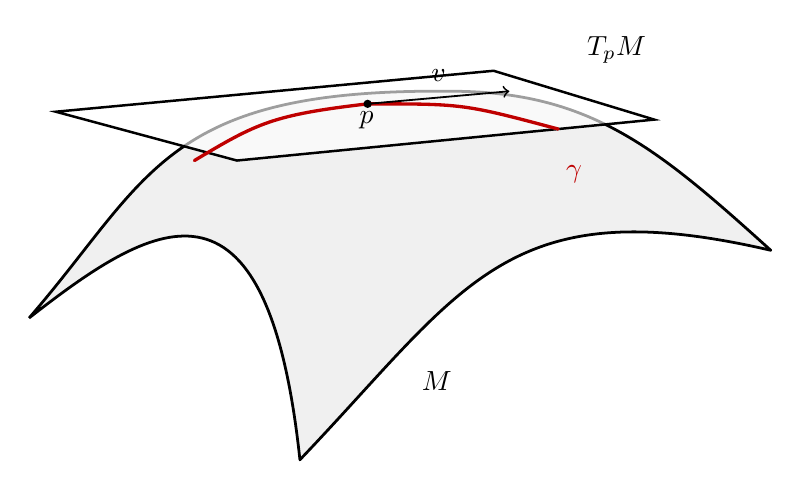
\begin{tikzpicture}[
    manifold/.style={
        draw=black,
        fill=gray!12,
        line width=1pt,
        line join=round
    },
    tangentplane/.style={
        draw=black,
        fill=white,
        fill opacity=0.62,
        draw opacity=1,
        line width=0.9pt
    },
    curve/.style={
        draw=red!75!black,
        line width=1.2pt,
        line cap=round
    },
    vector/.style={
        ->,
        draw=black,
        line width=0.65pt
    }
]

% Curved sheet M
\draw[manifold]
    (-4.9,-0.4)
    .. controls (-3.36,1.38) and (-3.2,2.52) ..
    (0.46,2.48)
    .. controls (2.24,2.48) and (3.1,1.74) ..
    (4.52,0.46)
    .. controls (1.16,1.24) and (0.64,0) ..
    (-1.46,-2.2)
    .. controls (-1.88,1.74) and (-3.36,0.8) ..
    (-4.9,-0.4);

% Point p
\coordinate (p) at (-0.6,2.32);

% Tangent plane T_p M
\draw[tangentplane]
    (-4.56,2.22)
    -- (1,2.74)
    -- (3.04,2.12)
    -- (-2.26,1.6)
    -- cycle;

% Curve gamma through p
\draw[curve]
    (-2.8,1.6)
    .. controls (-2,2.08) and (-1.8,2.18) ..
    (p)
    .. controls (0.62,2.32) ..
    (1.82,2);

% Tangent vector v = gamma-dot(0)
\draw[vector]
    (p) -- (1.2,2.48)
    node[midway,above=2pt] {\(v\)};

% Labels
\node[black] at (0.28,-1.2) {\(M\)};
\node[black] at (2.56,3) {\(T_pM\)};
\node[xshift=0.27cm, yshift=-0.51cm, black, above left=2pt] at (p) {\(p\)};
\node[red!75!black] at (2.02,1.42) {\(\gamma\)};

\fill[black] (p) circle (1.5pt);

% Curve notation

\end{tikzpicture}
\end{center}

What's good about the tangent space is that, a smooth map \(
  (M,p) \xlongrightarrow{f} (N,q)
\) naturally induces a map \(
  T_pM \xlongrightarrow{df_p} T_qN
\). To see this, we first define the \emph{push-forward} map \(f^\sharp:\cal{C}_p \longrightarrow \cal{C}_q\) by \[
  f^\sharp(\c) = f\circ\c.
\]
In this way, \(f^\sharp\) preserves the tangency, i.e.\ if \(\c_a\sim\c_b\), then \(f^\sharp(\c_a)\sim f^\sharp(\c_b)\). Then the map \(df_p\) is induced by the commutative diagram \[
  \begin{tikzcd}[column sep=huge]
    \cal{C}_p \ar[']{d}{[\,\cdot\,]_\sim} \ar{r}{f^\sharp} & \cal{C}_q \ar{d}{[\,\cdot\,]_\sim} \\
    T_pM \ar[dashed]{r}{df_p} & T_qN
  \end{tikzcd}.
\]
% such that\[
%   \begin{tikzcd}[column sep=huge,row sep=large]
%     T_p M \ar{r}{df_p} \ar{d}{\Phi_\varphi} &[4em] T_qN \ar{d}{\Phi_\psi} \\
%     \R^m \simeq T_{\Phi_\varphi(p)}\R^m
%     \ar{r}{D(\Phi_\psi\circ f\circ \Phi_\varphi^{-1})(p)} & T_{\Phi_\psi(f(p))}\R^n \simeq \R^n
%   \end{tikzcd}
%   \quad\text{commutes.}
% \]

\begin{definition}[\emph{differential}]
  Let \(M\), \(N\) be smooth manifolds and \(f:M\to N\) be smooth. For each \(p\in M\), we define the \emph{differential of \(f\) at \(p\)} by the linear map \(df_p:T_pM\to T_{f(p)}N\) given by \[
    df_p([\gamma]) = [f\circ\gamma].
  \]
\end{definition}

\begin{example}
  Let \(f:U\longrightarrow V\) be a smooth map between open subsets of \(\R^m\) and \(\R^n\). For \(p\in U\), we have \[
    \c_a \sim \c_b
    \quad\Longleftrightarrow\quad
    \frac{d}{dt} \c_a(t)\Big|_{t=0} = \frac{d}{dt} \c_b(t)\Big|_{t=0}
  \] because the chart is taken to be the identity, i.e.\ \((\varphi = \id,U,\R^m)\) and \((\psi = \id,V,\R^n)\).
  \begin{roof}
    In this way, we obtain \emph{canonical identifications} \(\Phi_\f:T_p\R^m \xlongrightarrow{\simeq} \R^m\) and \(\Phi_\psi:T_q\R^n \xlongrightarrow{\simeq} \R^n\) by \[
    [\c]_\sim \longmapsto \frac{d}{dt}\c(t)\Big|_{t=0}.
  \]
    In addition, \(U\xlongrightarrow{f}V\) induces \[
      \begin{tikzcd}
        & \cal{C}_p \ar[']{d}{[\,\cdot\,]_\sim} \ar{r}{f^\sharp} & \cal{C}_q \ar{d}{[\,\cdot\,]_\sim} & \\
        \R^m \simeq \hspace{-3em} & T_pU \ar{r}{df_p} & T_qV & \hspace{-3em} \simeq \R^n
      \end{tikzcd},
    \] here \(df_p\) is nothing but the Jacobian \(D f(p)\). Concretely, let \(\a\in\R^m\) be represented by \(\c_\a(t) = p + t\a\), then since \[
      \frac{d}{dt} \id(f\circ\c_\a(t))\Big|_{t=0}
      = \frac{d}{dt} f(p + t\a)\Big|_{t=0}
      = Df(p)\a,
    \] we compute carefully \begin{align*}
      df_p(\Phi_\f^{-1}(\a))
      = df_p([\c_\a])
      = [f\circ\c_\a]
      = \Phi_\psi^{-1}\bigg(\frac{d}{dt} \id(f\circ\c_\a(t))\Big|_{t=0}\bigg)
      = \Phi_\psi^{-1}\Big(Df(p)\a\Big),
    \end{align*}
    identifying \(df_p\) with the Jacobian \(Df(p)\).
  \end{roof}
\end{example}

% \begin{proposition}
%   Under a chart \((\f,U,V)\), the identification \(\Phi_\f:T_pM\longrightarrow\R^m\) defined by \[
%     [\c]_\sim \longmapsto \frac{d}{dt}\f\circ\c(t)\Big|_{t=0}
%   \] is a well-defined linear isomorphism. Moreover, such identification is independent of the choice of the chart.
% \end{proposition}
% \begin{proof}
%   \begin{itemize}
%     \item Well-definedness and injectivity follow the definition of \(\sim\).
%     \item Surjectivity. For any \(\y = \Phi_\f([\c])\in\R^n\), we take \(\gamma(t) = \f^{-1}(\f(p) + t\y)\), then \begin{align*}
%       \frac{d}{dt}\f\circ\c(t)\Big|_{t=0}
%       = \frac{d}{dt}(\f(p) + t\y)\Big|_{t=0}
%       = \y.
%     \end{align*}
%     \item We equip \(T_pM\) with some linear structure such that \(\Phi_\f\) is linear.
%   \end{itemize}
%   Now we show this linear structure is not dependent on the choice of the chart.
%   \begin{roof}
%     Let \((\f_1,U_1,V_1)\) be another chart at \(p\), then by the chain rule, we have \begin{align*}
%       \Phi_{\f_1}([\c])
%       = \frac{d}{dt}\f_1\circ\c(t)\Big|_{t=0}
%       = \frac{d}{dt}(\f_1\circ\f^{-1})(\f\circ\c(t))\Big|_{t=0}
%       = D(\f_1\circ\f^{-1})(\f(p))\ \Phi_\f([\c]),
%     \end{align*} in which the Jacobian is a linear isomorphism.
%   \end{roof}
% \end{proof}

% To clear confusion brought by the notation, we compute the following example explicitly using \(\Phi_\varphi\).

% \begin{example}\label{ex:diff_grad}
%   Let \(f:\R^m\to\R\) be a smooth function, choose the global charts \((\varphi = \id,\R^m,\R^m)\) and \((\psi = \id,\R,\R)\).
%   For each \(p\in\R^m\), pick \(\a\in\R^m\) represented by \(\gamma_\a(t) = p + t\a\), then since \begin{align*}
%     \frac{d}{dt}\id(f\circ\gamma_\a(t))\Big|_{t=0}
%     = \frac{d}{dt} f(p + t\a)\Big|_{t=0}
%     = \sum_{i=1}^m \frac{\partial f}{\partial x_i}(p)\a_i
%     = \nabla f(p)\a,
%   \end{align*} we have \begin{align*}
%     df_p(\Phi_\varphi^{-1}(\a))
%     = df_p([\gamma_\a])
%     = [f\circ\gamma_\a]
%     &= \Phi_\psi^{-1}\left(
%       \frac{d}{dt}\id(f\circ\gamma_\a(t))\Big|_{t=0}
%     \right)
%     = \Phi_\psi^{-1}\Big(
%       \nabla f(p)\a
%     \Big),
%   \end{align*} which wraps a matrix multiplication, where \(\nabla f(p)\) is treated as a \(1\times m\) matrix.
%   Hence we recover \(df_p\longleftrightarrow \nabla f(p)\), i.e. \(\Phi_\varphi\circ df_p\circ\Phi_\psi^{-1} = \nabla f(p)\).
% \end{example}

% \begin{example}\label{ex:diff_jacobian}
%   Let \(F:\R^m\to\R^n\) be a smooth function, choose the global charts \((\varphi = \id,\R^m,\R^m)\) and \((\psi = \id,\R^n,\R^n)\).
%   For each \(p\in\R^m\), pick \(\a\in\R^m\longleftrightarrow[\gamma_\a]\in T_p\R^m\) as in Example~\ref{ex:diff_grad} to get \begin{align*}
%     dF_p(\Phi_\varphi^{-1}(\a))
%     = d\begin{pmatrix}
%       F_1 \\
%       \vdots \\
%       F_n
%     \end{pmatrix}_p([\gamma_\a])
%     = \Phi_\psi^{-1}\bigg(\begin{pmatrix}
%       \nabla F_1(p) \\
%       \vdots \\
%       \nabla F_n(p)
%     \end{pmatrix}\a\bigg)
%     = \Phi_\psi^{-1}\Big(DF(p)\a\Big),
%   \end{align*} which again wraps a matrix multiplication,
%   where \(DF(p)\) is the \(n\times m\) Jacobian matrix of \(F\) at \(p\).
%   Hence we recover \(dF_p\longleftrightarrow DF(p)\).
% \end{example}

In general, if \((\f_1,U_1,V_1)\) and \((\f_2,U_2,V_2)\) are two charts centered at \(p\in M\) i.e\ \(\f_1(p) = 0 = \f_2(p)\), then \[
    \begin{tikzcd}
    & U_1\cap U_2 \ar[']{dl}{\f_1} \ar{dr}{\f_2} & \\
    V_1 \ar{rr}{\f_{12}} && V_2
    \end{tikzcd}
    \quad\text{induces}\quad
    \begin{tikzcd}
    & T_pM \ar[']{dl}{(d\f_1)_p}[']{\simeq} \ar{dr}{(d\f_2)_p}[']{\simeq} & \\
    \R^m \simeq T_0V_1 \ar{rr}{(d\f_{12})_0} && T_0V_2 \simeq \R^m
    \end{tikzcd}.
  \]

Since \((d\f_1)_p\) is a bijection, we can identify \(T_p M\simeq\R^m\) through \[
    T_pM \xlongrightarrow{(d\f_1)_p} T_0V_1 \xlongrightarrow{\Phi_\id} \R^m,
\] and equip \(T_pM\) with a vector space structure such that \(T_pM\xlongrightarrow{(d\f_1)_p} T_0V_1\) is linear. Note that since the Jacobian \((d\f_{12})_0\) is a linear isomorphism, the linearity of \((d\f_2)_p\) is equivalent to the linearity of \((d\f_1)_p\).

\begin{theorem}[Chain rule]
  Let \(f:M\to N\) and \(g:N\to P\) be smooth maps, then for each \(p\in M\), we have \[
    d(g\circ f)_p = dg_{f(p)} \circ df_p.
  \]
\end{theorem}
\begin{proof}
  Let \([\c]_\sim\in T_pM\), then \[
    df_p([\c]_\sim) = [f\circ\c]_\sim \in T_{f(p)}N,
  \]
  applying \(dg_{f(p)}\) gives \begin{align*}
    dg_{f(p)}\circ df_p([\c]_\sim)
    = dg_{f(p)}([f\circ\c]_\sim)
    = [g\circ (f\circ\c)]_\sim
    = [(g\circ f)\circ\c]_\sim
    = d(g\circ f)_p([\c]_\sim).
  \end{align*}
\end{proof}

The following is an analogy of the Jacobian being invertible for a diffeomorphism.
\begin{proposition}
  Let \(f:M\to N\) be a smooth diffeomorphism, then for each \(p\in M\), \(df_p:T_pM\to T_{f(p)}N\) is a linear isomorphism.
\end{proposition}
\begin{proof}
  If \(f\) is a smooth diffeomorphism, then \(f^{-1}\) induces a linear map \(df^{-1}_{f(p)}:T_{f(p)}N\to T_pM\) such that by the chain rule, \[
    df^{-1}_{f(p)}\circ df_p
    = d(f^{-1}\circ f)_p
    = \id_{T_pM}
    = d(f\circ f^{-1})_p
    = df_p\circ df^{-1}_{f(p)},
  \] showing that \(df_p\) is invertible.
\end{proof}

\begin{corollary}
  If \(\dim M = m\), then \(T_p M\) is an \(m\)-dimensional vector space.
\end{corollary}
\begin{proof}
  Consider a chart \((\f,U,V)\) at \(p\), then follow the linear isomorphism \(T_pM \xlongrightarrow{d\f_p} T_0V \simeq \R^m\).
\end{proof}

% Let's restate the inverse function theorem in the case of Euclidean spaces.
% \begin{proposition}[Inverse function theorem]
%   If \(U\), \(V\) are open subsets of \(\R^m\) and \(f:(U,0)\to(V,0)\). If \(df_0:T_0U\to T_0V\) is invertible, then \(f\) is a local diffeomorphism.
% \end{proposition}

\begin{theorem}[Inverse function theorem]
  Let \(M\), \(N\) be smooth manifolds and \(f:M\to N\) be smooth. If \(df_p:T_pM\to T_{f(p)}N\) is an isomorphism, then \(f\) is a local diffeomorphism at \(p\).
\end{theorem}

\begin{example}
  Let \(f:S^1\to S^1\) be the doubling map \(e^{i\theta}\mapsto e^{i2\theta}\). Here \(f\) is a local diffeomorphism, but not a global diffeomorphism.
\end{example}

Now, since we have fully identified \(T_pM\) with \(\R^m\), we can drop the identification maps and directly consider \(T_pM\) as a vector space.

\begin{proposition}[Basis for \(T_pM\)]
  Let \(M\) be a smooth manifold under a smooth chart \((\varphi,U,V)\). If \(\{x_1,\ldots,x_m\}\) constitutes a basis of \(\R^m\), then \[
    \left\{
      \dfrac{\pa}{\pa x_1}\bigg|_p, \ldots, \dfrac{\pa}{\pa x_m}\bigg|_p
    \right\},
    \quad\text{where}\quad
    \frac{\pa}{\pa x_i}\bigg|_p
    := (d\f_p)^{-1}(x_i),
  \] constitutes a basis for \(T_pM\).
\end{proposition}
\begin{proof}
  Since \((d\f_p)^{-1}\) is a linear isomorphism, it maps a basis of \(\R^m\) to a basis of \(T_pM\).
\end{proof}

Consequently, a vector \(v\in T_pM\) can be written \[
  v = \sum_{i=1}^m v_i \frac{\pa}{\pa x_i}\bigg|_p,
\] where \(v_i\in\R\) are the components of \(v\).

We call each \(\dfrac{\pa}{\pa x_i}\bigg|_p\) the \emph{\(i\)-th partial derivative}, it enjoys the property that \begin{align*}
  df_p\bigg(\frac{\pa}{\pa x_i}\bigg|_p\bigg)
  = df_p\big((d\f_p)^{-1}(x_i)\big)
  = d(f\circ\f^{-1})_{\f(p)}(x_i)
  = D(f\circ\f^{-1})(\f(p))\cdot x_i
  = \frac{\pa f}{\pa x_i}\bigg|_{x=p}.
\end{align*}

% \begin{example}\label{ex:diff_partial_grad}
%   Let \(f:\R^m\to\R\) be a smooth map and \(p\in\R^m\) under the global charts \((\varphi = \id,\R^m,\R^m)\) and \((\psi = \id,\R,\R)\) respectively. Then by Example~\ref{ex:diff_grad} we have \begin{align*}
%     df_p\left(\frac{\pa}{\pa x_i}\bigg|_p\right)
%     = df_p(\Phi_\varphi^{-1}(\e_i))
%     = \Phi_\psi^{-1}\Big(\nabla f(p)\e_i\Big)
%     = \Phi_\psi^{-1}\left(
%       \frac{\pa f}{\pa x_i}\bigg|_{x = p}
%     \right),
%   \end{align*} which wraps the \(i\)-th partial derivative of \(f\) at \(p\).
% \end{example}

% \begin{example}
%   Let \(F:\R^m\to\R^n\) be a smooth map and \(p\in\R^m\), \(F(p)\in\R^n\) under the global charts \((\varphi = \id,\R^m,\R^m)\) and \((\psi = \id,\R^n,\R^n)\) respectively. Then by Example~\ref{ex:diff_jacobian} we have \begin{align*}
%     dF_p\left(\frac{\pa}{\pa x_i}\bigg|_p\right)
%     = dF_p\left(\Phi_\varphi^{-1}(\e_i)\right)
%     = \Phi_\psi^{-1}\Big(DF(p)\e_i\Big)
%     = \Phi_\psi^{-1}\left(
%       \frac{\pa F}{\pa x_i}\bigg|_{x=p}
%     \right),
%   \end{align*} which wraps the \(i\)-th column of the Jacobian of \(F\) at \(p\).
% \end{example}

% If \(\dim M = 1\), we write \(\dfrac{d}{dx}\bigg|_p := \dfrac{\pa}{\pa x_1}\bigg|_p\) for the unique basic element of \(T_pM\).

% From now on, we omit writting \(\Phi_\varphi^{-1}\) and \(\Phi_\psi^{-1}\) when we identify \(T_pM\longleftrightarrow\R^m\) and \(T_{f(p)}N\longleftrightarrow\R^n\), we abuse notations to mean \[
%   dF_p = DF(p),
%   \quad
%   dF_p\left(\frac{\pa}{\pa x_i}\bigg|_p\right) = \frac{\pa F}{\pa x_i}\bigg|_{x=p}.
% \]

\section{Submersion and Immersion}

This section follows Guillemin, Pollack: Chapter 1.3 and 1.4

\begin{definition}[\emph{submersion}, \emph{immersion}]
  Let \(M\), \(N\) be smooth manifolds and \(f:M\to N\) be a smooth map. We say \(f\) is \begin{itemize}
    \item a \emph{submersion at \(p\)} if \(df_p:T_pM\to T_{f(p)}N\) is surjective.
    \item an \emph{immersion at \(p\)} if \(df_p:T_pM\to T_{f(p)}N\) is injective.
  \end{itemize}
\end{definition}
Clearly, a submersion implies \(\dim M \geq \dim N\), while an immersion implies \(\dim M \leq \dim N\).

\begin{example}[Canonical submersion]
  Consider the projection \(\pi:\R^m\to\R^n\) for \(m\geq n\) given by \[
    \pi(x_1,\ldots,x_m) = (x_1,\ldots,x_n).
  \]
\end{example}
\begin{example}[Canonical immersion]
  Consider the inclusion \(\iota:\R^m\to\R^n\) for \(m\leq n\) given by \[
    \iota(x_1,\ldots,x_m) = (x_1,\ldots,x_m,0,\ldots,0).
  \]
\end{example}
In this view, a submersion is locally like a projection, while an immersion is locally like an inclusion. The following theorem is a analogy of the implicit function theorem.
\begin{theorem}[Canonical submersion theorem]
  Let \(M\), \(N\) be smooth manifolds and \(f:M\to N\) be a submersion at \(p\in M\). Then there exists charts \((\varphi_1,U_1,V_1)\) at \(p\) and \((\psi_1,X_1,Y_1)\) at \(f(p)\) such that \[
    \psi_1\circ f\circ\varphi_1^{-1} = \pi\restriction_{V_1}:
    V_1\subset\R^m\longrightarrow Y_1\subset\R^n.
  \]
\end{theorem}
\begin{proof}
  Choose some charts \((\varphi,U,V)\) at \(p\) and \((\psi,X,Y)\) at \(f(p)\), write \(F = \psi\circ f\circ\varphi^{-1}\), then \begin{align*}
    dF_{\varphi(p)} = d\psi_{f(p)}\circ df_p\circ d\varphi^{-1}_{\varphi(p)}:T_{\varphi(p)}V\longrightarrow T_{\psi(f(p))}Y
  \end{align*}
  As \(T_{\varphi(p)}V\simeq\R^m\) and \(T_{\psi(f(p))}Y\simeq\R^n\), \(dF_{\varphi(p)}\) is just the Jacobian \(\left(\dfrac{\pa F_i}{\pa x_j}\right)_{1\leq i \leq n, 1\leq j \leq m}\).
  The surjectivity of \(df_p\) implies the surjectivity of \(dF_{\varphi(p)}\), hence \(\rank dF_{\varphi(p)} = n\).
  \begin{center}
    \begin{tikzpicture}[
      sizearrow/.style={
          <->,
          line width=0.5pt
      }
    ]
      \node at (0,0) {
        \(
          dF_{\varphi(p)} = \begin{pmatrix}
            \phantom{
              \dfrac{\pa F_1}{\pa x_1}
              \dfrac{\pa F_1}{\pa x_2}
              \dfrac{\pa F_1}{\pa x_3}
              \dfrac{\pa F_1}{\pa x_4}
              \dfrac{\pa F_1}{\pa x_5}
              \dfrac{\pa F_1}{\pa x_6}
              \dfrac{\pa F_1}{\pa x_m}}\\
            \phantom{
              \dfrac{\pa F_2}{\pa x_1}
              \dfrac{\pa F_2}{\pa x_2}
              \dfrac{\pa F_2}{\pa x_3}
              \dfrac{\pa F_2}{\pa x_4}
              \dfrac{\pa F_2}{\pa x_5}
              \dfrac{\pa F_2}{\pa x_6}
              \dfrac{\pa F_2}{\pa x_m}}\\
            \phantom{
              \dfrac{\pa F_3}{\pa x_1}
              \dfrac{\pa F_3}{\pa x_2}
              \dfrac{\pa F_3}{\pa x_3}
              \dfrac{\pa F_3}{\pa x_4}
              \dfrac{\pa F_3}{\pa x_5}
              \dfrac{\pa F_3}{\pa x_6}
              \dfrac{\pa F_3}{\pa x_m}}
          \end{pmatrix}
        \)
      };
      \draw[sizearrow] (3.9,1.3) -- (3.9,-1.3) node [midway,right] {\(n\)};
      \draw[sizearrow] (-2,-1.5) -- (3.65,-1.5) node [midway,below] {\(m\)};

      \draw[sizearrow, red!75!black] (1,1.2) -- (1,-1.2) node [midway,right] {\(n\)};
      \draw[sizearrow, red!75!black] (-1.7,1.5) -- (0.7,1.5) node [midway,above] {\(n\)};

      \node[red!75!black] at (-0.5,0) {
        \(
          \begin{pmatrix}
            \vspace{55pt}\hspace{60pt}
          \end{pmatrix}
        \)
      };

      \node[red!75!black] at (-0.525,0) {\(A\)};
      \node[black] at (2.35,0) {\(*\)};
    \end{tikzpicture}
  \end{center}
  By rearranging the basis, we can assume the left \(n\times n\) block \(A\) of the Jacobian is invertible.

  Define \(G:V\subset\R^m\to\R^n\) by \[
    G(x_1,\ldots,x_m) = (F_1,(\x),\ldots,F_n(\x),x_{n+1},\ldots,x_m).
  \] We compose \(\varphi\) with \(G\) to obtain \(\varphi_1 = G\circ\varphi\), now we have \[
    \begin{tikzcd}[column sep=huge,row sep=large]
         U \ar{r}{f} \ar{d}{\varphi} \ar[bend right=60,swap]{dd}{\varphi_1} & X \ar{d}{\psi} \\
         V \ar{r}{F}[swap]{\psi\circ f\circ\varphi^{-1}} \ar{d}{G} & Y \\
      \R^m \ar[dashrightarrow,bend right=30]{ur}{F\circ G^{-1}}[swap]{\psi\circ f\circ\varphi_1^{-1}}
    \end{tikzcd},
  \] in particular we have
  \[
    \psi\circ f\circ\varphi_1^{-1}
    = F\circ G^{-1}
    = \pi\restriction_{G(V)}.
  \] 
  Now \((\varphi_1,U_1,V_1)\) is indeed a chart at \(p\) because \begin{center}
    \begin{tikzpicture}[
      sizearrow/.style={
          <->,
          line width=0.5pt
      }
    ]
      \node at (-0.25,-0.68) {
        \(
          dG_{\varphi(p)} = \begin{pmatrix}
            \vspace{103pt}\hspace{133pt}
          \end{pmatrix}
        \)
      };

      \draw[sizearrow, red!75!black] (1,1.2) -- (1,-1.2) node [midway,right] {\(n\)};
      \draw[sizearrow, red!75!black] (-1.7,1.5) -- (0.7,1.5) node [midway,above] {\(n\)};

      \draw[sizearrow] (1,-1.2) -- (1,-2.6) node [midway,left] {\(m-n\)};
      \draw[sizearrow] (1.2,-2.8) -- (2.95,-2.8) node [midway,below] {\(m-n\)};

      \node[red!75!black] at (-0.5,0) {
        \(
          \begin{pmatrix}
            \vspace{55pt}\hspace{60pt}
          \end{pmatrix}
        \)
      };

      \node[black] at (2.05,-1.9) {
        \(
          \begin{pmatrix}
            \vspace{25pt}\hspace{35pt}
          \end{pmatrix}
        \)
      };

      \node[red!75!black] at (-0.525,0) {\(A\)};
      \node[black] at (2.05,-1.9) {\(I_{m-n}\)};
      \node[black] at (2.05,0) {\(*\)};
    \end{tikzpicture}
  \end{center}
  is invertible, and inverse function theorem shows \(G\) is a local diffeomorphism at \(\varphi(p)\).
\end{proof}

\begin{theorem}[Canonical immersion theorem]
  Let \(M\), \(N\) be smooth manifolds and \(f:M\to N\) be an immersion at \(p\in M\). Then there exists charts \((\varphi_1,U_1,V_1)\) at \(p\) and \((\psi_1,X_1,Y_1)\) at \(f(p)\) such that \[
    \psi_1\circ f\circ\varphi_1^{-1} = \iota\restriction_{V_1}:
    V_1\subset\R^m\longrightarrow Y_1\subset\R^n.
  \]
\end{theorem}
\begin{proof}
  Similar to the previous proof.
\end{proof}

To summarize, we have a local picture between \(f:M\to N\) and \(df_p:T_pM\to T_{f(p)}N\) \[
  \begin{array}{c@{\qquad}c@{\qquad}c}
  f: M \to N & & df_p: T_pM \to T_{f(p)}N \\[4pt]
  \text{local diffeomorphism} & \Longleftrightarrow & \text{isomorphism} \\[4pt]
  \text{canonical submersion}\approx\pi & \Longleftrightarrow & \text{surjection} \\[4pt]
  \text{canonical immersion}\approx\iota & \Longleftrightarrow & \text{injection}
  \end{array}
\]

\section{Embedding and Smooth Submanifolds}
The next question is, what happens globally? Let's look at a few examples of bad global behaviors.

\begin{example}
  Consider the maps \(\R\to\R^2\) with graphs \begin{center}
    \vspace{-14pt}
    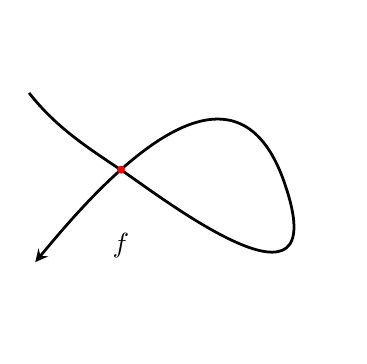
\begin{tikzpicture}
      \draw[-stealth, line width=1pt]
        (0.4828,2.8542)
          .. controls (0.8240,2.4200) and (1.2028,2.1742) .. (1.6618,1.8686)
          .. controls (2.1206,1.5628) and (4.4018,-0.2148) .. (3.7218,1.7252)
          .. controls (3.0418,3.6652) and (1.2634,1.5502) .. (0.5618,0.7052);

      \fill[red] (1.65,1.88) circle[radius=0.05];

      \node at (1.65,1.2) [below] {\(f\)};
    \end{tikzpicture}
    \qquad
    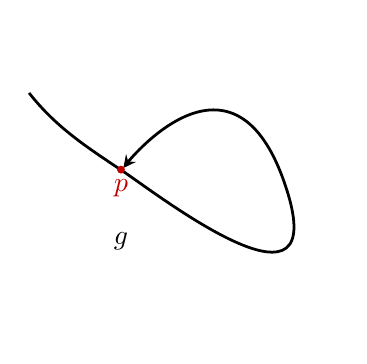
\begin{tikzpicture}
      \draw[-stealth, line width=1pt]
        (0.4828,2.8542)
          .. controls (0.8240,2.4200) and (1.2028,2.1742) .. (1.6618,1.8686)
          .. controls (2.1206,1.5628) and (4.4018,-0.2148) .. (3.7218,1.7252)
          .. controls (3.0418,3.6652) and (1.68,1.9) .. (1.68,1.9);

      \fill[red!75!black] (1.65,1.88) circle[radius=0.05] node [below] {\(p\)};
      \node at (1.65,1.2) [below] {\(g\)};
    \end{tikzpicture}
    \vspace{-20pt}
  \end{center}
  We see \(f\) could be an immersion, but definitely not injective. Then we construct \(g\) by making \(p = \lim_{t\to\infty} g(t)\), so \(g\) is injective, but still, the topology of the image is not like \(\R\), any neighbourhood of \(p\) always contain two branches. 

  We would like the subspace topology of \(f(M)\) induced by \(N\) to be the same as the topology of \(M\).
\end{example}

\begin{example}
  Consider the map \(f:\R\to\S^1\times\S^1\) by \[
    f(t) = (e^{it},e^{i\sqrt{2}t}).
  \]
  We visualize the torus using fundamental polygon with edge identification \(ab^{-1}a^{-1}b\).
  \begin{center}
    \begin{tikzpicture}[
    spacefilling/.style={postaction={
        pattern={
            Lines[
                angle=45,
                distance=3pt,
                line width=1pt
            ]
        },
        pattern color=blue!75!black,
    }},
    axis/.style={
        -Stealth,
        black,
        line width=1pt
    }
]
    \draw[spacefilling, line width=1pt] (0,0) rectangle (3,3);

    
    \draw[axis] (0,3) -- (1.65,3);
    \draw[axis] (0,0) -- (1.65,0);

    \draw[axis] (0,0) -- (0,1.45);
    \draw[axis] (0,0) -- (0,1.85);

    \draw[axis] (3,0) -- (3,1.45);
    \draw[axis] (3,0) -- (3,1.85);

    \node[blue!75!black] at (4.3,0.7) {slope \(=\sqrt{2}\)};
\end{tikzpicture}
  \end{center}
  Since the slope is irrational, \(f(\R)\) is dense in \(\S^1\times\S^1\), hence the subspace topology of \(f(M)\) induced by \(N\) is not the same as the topology of \(M\).
\end{example}

\begin{definition}
  Let \(M\), \(N\) be smooth manifolds and \(f:M\to N\) be a smooth map. We say \(f\) is an \emph{embedding} if \begin{itemize}
    \item \(f\) is an immersion, and
    \item \(f:M\to f(M)\) is a homeomorphism
  \end{itemize}
  where \(f(M)\subset N\) is endowed the subspace topology.
\end{definition}

\begin{proposition}
  If \(f:M\to N\) is an injective immersion and \(M\) is compact, then \(f\) is an embedding.
\end{proposition}
\begin{proof}
  Since \(f:M\to f(M)\) is bijective, we have its inverse \(f^{-1}:f(M)\to M\). Now it suffices to show that \(f^{-1}\) is continuous. Let \(F\subset M\) be closed, hence compact. Then by continuity, \(f(F)\) is compact. By Hausdorff, \(f(F)\) is closed.
\end{proof}

The concept of embedding is closely related to the concept of submanifolds, which are subsets of manifolds, which itself are manifolds.

\begin{definition}
  A subset \(S\subset M\) is a \emph{smooth submanifold of \(M\)} if there exists some \(k\) such that for each \(p\in S\), there is an \emph{adapted chart} \((\varphi,U,V)\) around \(p\in M\) such that \[
    \varphi(U\cap S) = V\cap \underbrace{(\R^k\times\{0\}^{m-k})}_{\text{a slice}} = \{x\in\varphi(U)\mid x_{k+1} = \cdots = x_m = 0\}.
  \]
  We define the \emph{dimension} and \emph{codimension} of \(S\) by \(\dim S = k\) and \(\codim S = m - k\).
\end{definition}

\begin{center}
  \begin{tikzpicture}[
    manifold/.style={
        draw=black,
        fill=gray!10,
        line width=1pt
    },
    submanifold/.style={
        draw=red!75!black,
        fill=red!25,
        fill opacity=0.7,
        draw opacity=1,
        line width=2pt
    },
    chart/.style={
        draw=blue!75!black,
        fill=blue!25,
        fill opacity=0.7,
        draw opacity=1,
        line width=1pt
    },
    slice/.style={
        red!85!black,
        line width=2pt
    },
    chartarrow/.style={
        ->,
        red!75!black,
        line width=0.5pt
    },
    axis/.style={
        -Stealth,
        black,
        line width=1pt
    }
]

% M
\draw[manifold]
    plot[smooth cycle, tension=0.75] coordinates {
        (-3.50,1.45)
        (-3.20,2.15)
        (-2.45,2.65)
        (-1.45,2.78)
        (-0.35,2.68)
        (0.55,2.45)
        (1.05,1.95)
        (0.90,1.35)
        (0.15,1.00)
        (-0.95,0.92)
        (-2.15,1.00)
        (-3.00,1.12)
    };
\node[black] at (0.90,2.70) {\(M\)};

% S in M
\draw[submanifold]
    (-2.60,1.38) .. controls (-1.75,1.70) and (-0.55,1.92) .. (0.65,2.12);
\node[red!75!black] at (0.42,1.75) {\(S\)};

% U in M
\draw[chart]
    plot[smooth cycle, tension=0.75] coordinates {
        (-1.85,1.68)
        (-1.55,2.05)
        (-1.00,2.18)
        (-0.38,2.12)
        (0.00,1.86)
        (-0.18,1.55)
        (-0.75,1.45)
        (-1.38,1.48)
    };

\node[blue!80!black] at (-2.15,1.85) {\(U\)};

% Point p
\fill[black] (-1.02,1.82) circle (1.4pt);
\node[black, above] at (-1.02,1.26) {\(p\)};

% V
\draw[chart, yshift=-10pt]  
    plot[smooth cycle, tension=0.75] coordinates {  
        (-2.05,-1.35)  
        (-1.85,-0.70)  
        (-1.35,-0.25)  
        (-0.62,-0.18)  
        (-0.05,-0.50)  
        ( 0.10,-1.10)  
        (-0.25,-1.60)  
        (-0.95,-1.75)  
        (-1.65,-1.65)  
    };
\node[blue!80!black] at (-2.4,-1.58) {\(V\)};

\draw[chartarrow, bend left=60]
    (-0.72,1.55) to
    node[midway,right] {\(\varphi\)}
    (-0.72,-1.05);
    
% R^k
\draw[axis] (-1.02,-1.3) -- (0.48,-1.3) node[right] {\(\R^k\)};
\draw[axis] (-1.02,-1.3) -- (-1.02,0.2) node[above] {\(\R^{m-k}\)};

% Slice image V cap (R^k x {0})
\draw[submanifold]
    (-1.7,-1.3) -- (-0.2,-1.3);

\end{tikzpicture}
\end{center}

\begin{example}
  \(S^n\) is a smooth submanifold of \(\R^{n+1}\) of \(\codim = 1\).
\end{example}

\begin{example}
  Given a smooth map \(f:M\to N\), the graph \[
    \Gamma(f) = \{(p,f(p))\mid p\in M\}
  \] is a smooth submanifold of \(M\times N\).
\end{example}

\begin{theorem}
  Let \(S\) be a smooth submanifold of \(M\) of \(\dim = k\). Then under the subspace topology, \begin{itemize}
    \item \(S\) is a smooth manifold of \(\dim = k\), and
    \item the inclusion \(\iota:S\to M\) is an embedding.
  \end{itemize}
\end{theorem}
\begin{proof}
  \begin{itemize}
    \item Let \(p\in S\), we compose adapted chart \((\varphi,U,V)\) with the projection \(\pi:\R^m\to\R^k\) to obtain a chart \((\pi\circ\varphi,U\cap S,\pi(V))\) of \(S\) at \(p\). The transition maps are smooth because they are just the restrictions of the transition maps of \(M\).
    \item The inclusion is clearly an immersion, and it is a homeomorphism onto its image because the subspace topology of \(S\) is the same as the topology of \(S\) as a manifold. 
  \end{itemize}
\end{proof}

\begin{theorem}
  Start with an embedding \(f:M\to N\), then \(f(M)\) is a smooth submanifold of \(N\).
\end{theorem}
\begin{proof}
  Let \(q\in f(M)\) and \(p\in M\) such that \(f(p) = q\). Since \(f\) is an immersion, the canonical immersion theorem gives charts \((\varphi_1,U_1,V_1)\) at \(p\) and \((\psi_1,X_1,Y_1)\) at \(q\) such that \[
    \psi_1\circ f\circ\varphi_1^{-1} = \iota\restriction_{V_1}:
    V_1\subset\R^m\longrightarrow Y_1\subset\R^n.
  \] 
  We show that \((\psi_1,X_1,Y_1)\) is an adapted chart at \(q\).
  Since \(f\) is homeomorphic onto \(f(M)\), \(f(U_1)\) is open in \(f(M)\).
  \begin{align*}
    \psi_1(X_1\cap f(M))
    = Y_1\cap\psi_1(f(M))
    = Y_1\cap\iota\circ\varphi_1(M)
    = Y_1\cap(\R^m\times\{0\}^{n-m})
  \end{align*}
\end{proof}

\section{Regular Values and Regular Value Theorem}

Now we turn to investigate submersion in global setting.

\begin{definition}
  Let \(M\), \(N\) be smooth manifolds and \(f:M\to N\) be a smooth map.
  \begin{itemize}
    \item A point \(p\in M\) is a \emph{regular point} if \(df_p\) is surjective. Otherwise, we call \(p\) a \emph{singular point}, or n m\emph{regular point}. Denote by \(C_f\) the set of singular points of \(f\).
    \item A point \(q\in N\) is a \emph{regular value} if all \(f^{-1}(q)\) are regular points. Otherwise, we call \(q\) a \emph{singular value}, or \emph{critical value}. Then \(f(C_f)\) is the set of singular values of \(f\).
  \end{itemize}
\end{definition}

\begin{example}
  Consider the function \(f:\R^{n+1}\to\R\) given by \[
    f(x_1,\ldots,x_{n+1}) = x_1^2 + \cdots + x_{n+1}^2.
  \]
  We compute the linear map \begin{align*}
    df_p &= (2x_1, \ldots, 2x_{n+1}): T_p\R^{n+1}\to T_{f(p)}\R \\
    df_p([\a]) &= \<(2x_1, \ldots, 2x_{n+1}),\a\>.
  \end{align*}
  Hence \(df_p\) is singular if and only if \(x_1 = \cdots = x_{n+1} = 0\), so \(\bf{0} = (0,\ldots,0)\in\R^{n+1}\) is the only singular point, and all other points are regular points.
  Correspondingly, \(f(\bf{0}) = 0\in\R\) is the only singular value, and all other values are regular values.
\end{example}

\begin{example}
  Let \(f:M\to N\) with \(\dim M < \dim N\), then \(df_p:T_pM\to T_{f(p)}N\) maps a lower-dimensional vector space to a higher-dimensional vector space, hence it cannot be surjective. Therefore, all points in \(M\) are singular points, and all values in \(f(M)\) are singular values.
\end{example}

\begin{theorem}[Regular Value Theorem]
  If \(q\in N\) is a regular value of \(f:M\to N\), then \(S = f^{-1}(q)\) is a smooth submanifold of \(M\) of \(\codim = n\). Morevoer, for each \(p\in S\), \(T_pS = \ker df_p\).
\end{theorem}
\begin{proof}
  Let \(p\in S = f^{-1}(q)\), we want to put a chart around \(p\) such that  when restricted, is the slice.
  Then the canonical submersion theorem gives charts \((\varphi_1,U_1,V_1)\)  centered at \(p\) and \((\psi_1,X_1,Y_1)\) centered at \(q\) with \[
      \psi_1\circ f\circ\varphi_1^{-1} = \pi\restriction_{V_1}:
      V_1\subset\R^m\longrightarrow Y_1\subset\R^n.
  \] 
  \begin{center}
      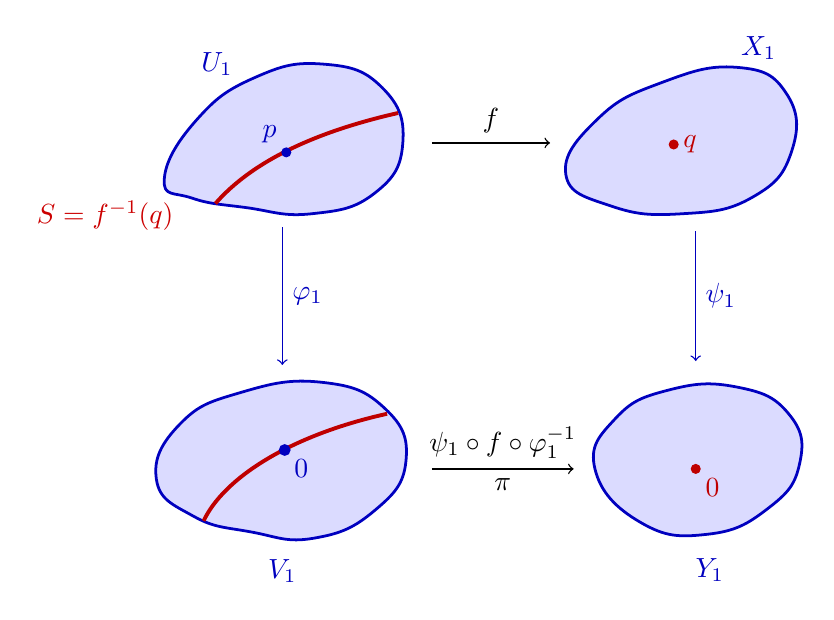
\begin{tikzpicture}[
    space/.style={
        draw=blue!75!black,
        fill=blue!20,
        fill opacity=0.7,
        draw opacity=1,
        line width=1pt
    },
    slice/.style={
        red!75!black,
        line width=1.4pt
    },
    maparrow/.style={
        ->,
        line width=0.5pt
    },
    bluearrow/.style={
        ->,
        blue!75!black,
        line width=0.5pt
    },
    bluepoint/.style={
        fill=blue!75!black,
        draw=blue!75!black
    },
    redpoint/.style={
        fill=red!75!black,
        draw=red!75!black
    },
]

% ------------------------------------------------
% U_1 neighborhood of p
% ------------------------------------------------
\draw[space]
    plot[smooth cycle, tension=0.8] coordinates {
        (-3.85,1.25)
        (-3.45,2.00)
        (-2.70,2.55)
        (-1.82,2.72)
        (-1.08,2.42)
        (-0.82,1.72)
        (-1.18,1.08)
        (-1.98,0.82)
        (-2.82,0.90)
        (-3.50,1.02)
    };

\node[blue!75!black] at (-3.18,2.72) {\(U_1\)};

% S slice in U_1
\draw[slice]
    (-3.2,0.95)
    .. controls (-2.85,1.35) and (-2.20,1.80) ..
    (-0.88,2.10);

\node[red!80!black] at (-4.6,0.8) {\(S=f^{-1}(q)\)};

% bluepoint p
\fill[bluepoint] (-2.30,1.6) circle (1.6pt);
\node[blue!75!black, above left] at (-2.30,1.6) {\(p\)};

% ------------------------------------------------
% X_1
% ------------------------------------------------
\draw[space]
    plot[smooth cycle, tension=0.8] coordinates {
        (1.25,1.32)
        (1.65,2.02)
        (2.45,2.48)
        (3.42,2.68)
        (4.05,2.35)
        (4.12,1.62)
        (3.62,1.03)
        (2.72,0.82)
        (1.82,0.92)
    };

\node[blue!75!black] at (3.70,2.92) {\(X_1\)};

\fill[redpoint] (2.62,1.70) circle (1.6pt);
\node[red!75!black, right] at (2.62,1.70) {\(q\)};

% f arrow
\draw[maparrow]
    (-0.45,1.72) -- (1.05,1.72)
    node[midway,above] {\(f\)};

% V_1
\draw[space]
    plot[smooth cycle, tension=0.8] coordinates {
        (-3.95,-2.55)
        (-3.65,-1.85)
        (-2.88,-1.45)
        (-1.85,-1.32)
        (-1.05,-1.65)
        (-0.78,-2.32)
        (-1.18,-2.95)
        (-1.95,-3.30)
        (-2.75,-3.22)
        (-3.48,-3.02)
    };

\node[blue!75!black] at (-2.35,-3.72) {\(V_1\)};

% slice in V_1
\draw[slice]
    (-3.35,-3.08)
    .. controls (-3.10,-2.55) and (-2.28,-2.00) ..
    (-1.02,-1.72);

% origin in V_1
\filldraw[blue!75!black, line width=1pt] (-2.32,-2.18) circle (1.6pt);
\node[blue!75!black, below right] at (-2.32,-2.18) {\(0\)};

% phi_1 arrow
\draw[bluearrow]
    (-2.35,0.65) -- (-2.35,-1.10)
    node[midway,right] {\(\varphi_1\)};

% ------------------------------------------------
% Y_1
% ------------------------------------------------
\draw[space]
    plot[smooth cycle, tension=0.8] coordinates {
        (1.62,-2.42)
        (1.88,-1.78)
        (2.55,-1.42)
        (3.42,-1.38)
        (4.08,-1.72)
        (4.22,-2.35)
        (3.82,-2.92)
        (3.05,-3.25)
        (2.20,-3.10)
    };

\node[blue!75!black] at (3.08,-3.70) {\(Y_1\)};

% origin in Y_1
\fill[redpoint] (2.90,-2.42) circle (1.6pt);
\node[red!75!black, below right] at (2.90,-2.42) {\(0\)};

% psi_1 arrow
\draw[bluearrow]
    (2.90,0.60) -- (2.90,-1.05)
    node[midway,right] {\(\psi_1\)};

% pi arrow
\draw[maparrow]
    (-0.45,-2.42) -- (1.35,-2.42)
    node[midway,above] {\(\psi_1\circ f\circ\varphi_1^{-1}\)}
    node[midway,below] {\(\pi\)};

\end{tikzpicture}
  \end{center}
  In particular, \(\varphi_1\circ f^{-1} = \pi^{-1}\circ\psi_1\), then \begin{align*}
      \varphi_1(U_1\cap f^{-1}(q))
      = V_1\cap\varphi_1\circ f^{-1}(q)
      = V_1\cap\pi^{-1}\circ\psi_1(q)
      = V_1\cap\pi^{-1}(0),
      = V_1\cap(\{0\}^n\times\R^{m-n}),
  \end{align*} so \(f^{-1}(q)\) is a smooth submanifold of \(M\) with \(\codim S = n\).

  For the other part, let \(\iota:S\to M\) be the inclusion, then for each   \(p\in S\), \[
      f\circ\iota(p) = q,
  \] meaning \(f\circ\iota:S\to N\) is a constant map, hence by the chain rule, \[
    d(f\circ\iota)_p = df_p\circ d\iota_p = 0,
  \] so \(T_pS = \im d\iota_p \subset\ker df_p\).
  Apply the rank-nullity theorem to the surjection \(dp_f:T_pM\to T_qN\), \[
    m - n = \dim T_pS
    \leq \dim\ker(df_p)
    = \dim T_pM - \dim T_qN = m - n,
  \] forcing \(\dim T_pS = \dim\ker df_p\), hence \(T_pS = \ker df_p\).
\end{proof}

\begin{homework}
  Let \(\cal{M}_n\) be the space of all \(n\times n\) real matrices and \[
    \Sym_n = \{A\in\cal{M}_n\mid A^\top = A\}
  \] to be the space of all \(n\times n\) symmetric matrices, which is an \(\frac{n(n+1)}{2}\)-dimensional vector subspace of \(\cal{M}_n\). It is also a smooth manifold trivially, diffeomorphic to \(\R^{\frac{n(n+1)}{2}}\).
  Next, we let \[
    O(n) = \{A\in\cal{M}_n\mid A^\top A = I\}
  \] to be the space of all \(n\times n\) orthogonal matrices. We show that \(O(n)\) is an \(\frac{n(n-1)}{2}\)-dimensional smooth submanifold of \(\cal{M}_n\).
  \begin{roof}
    Construct \(f:\cal{M}_n \to \Sym_n\) by \[
      f(A) = A^t A.
    \]
    We can identify \(T_A\cal{M}_n\simeq\cal{M}_n\) and \(T_{f(A)}\Sym_n\simeq\Sym_n\), to compute \begin{align*}
      df_A(B) = A^t B + B^t A.
    \end{align*}
    Check that \(I_n\in\Sym_n\) is a regular value of \(f\), then by the regular value theorem, \(f^{-1}(I_n) = O(n)\) is a smooth submanifold of \(\cal{M}_n\) with \(\codim\cal{M}_n = \dim\Sym_n = \frac{n(n+1)}{2}\), hence \[
      \dim O(n) = n^2 - \frac{n(n+1)}{2} = \frac{n(n-1)}{2}.
    \]
  \end{roof}
\end{homework}

As level sets at a regular value \(q\) gives a smooth manifold, we ask whether we can always find a regular value. This brings us to the next theorem.
\begin{definition}[\emph{measure zero}]
  Let \(M\) be a smooth manifold, then a subset \(Z\subset M\) is said to have \emph{measure zero} if for any chart \((\varphi,U,V)\) of \(M\), \(\varphi(Z\cap U)\) has measure zero in \(\R^m\).
\end{definition}

\begin{theorem}[Sard's theorem]
  Let \(M\), \(N\) be smooth manifolds and \(f:M\to N\) is a smooth map. Then \(f(C_f)\) has measure zero in \(N\).

  In other words, almost all points in \(N\) are regular values of \(f\).
\end{theorem}
\begin{proof}
  Left as a project.
\end{proof}

\begin{homework}
  Consider again the map \(f:\cal{M}_n\longrightarrow \Sym_n\) by \[
    f(A) = A^t A.
  \]
  Find all regular points, singular points, regular values and singular values of \(f\). Check Sard's theorem for this example.
\end{homework}

\section{Partitions of Unity}

This chapter mainly follows Warner.

To construct a partition of unity, we utilze smooth bump functions.
\begin{example}
  To construct a smooth bump function in \(\R^n\), we start with \[
    f_1(x) = \begin{cases}
      e^{-1/x} & x > 0 \\
      0 & x \leq 0
    \end{cases}
    \quad\text{and}\quad
    f_2(x) = \frac{f_1(x)}{f_1(x) + f_1(\eps-x)},\ \eps > 0.
  \]
  \[
    \begin{tikzpicture}[
    axis/.style={
        -Stealth,
        black,
        line width=1pt
    },
    bluegraph/.style={
        blue!75!black,
        line width=1pt,
        smooth
    },
    redgraph/.style={
        red!75!black,
        line width=1pt,
        smooth
    },
]

\draw[axis] (-3.2,0) -- (4.0,0) node[right] {\(x\)};
\draw[axis] (0,-1.1) -- (0,2.4) node[above] {\(y\)};

\draw[redgraph] (-3.0,0) -- (0,0);

\draw[bluegraph, domain=0.05:3.6, samples=200]
    plot (\x,{2.0*exp(-1/\x)});

\fill[black] (0,0) circle (1.2pt);

% Label
\node[above right] at (1.7,1.35) {\(f_1\)};
\node[below right] at (0,0) {\(0\)};

\end{tikzpicture}
    \qquad
    \begin{tikzpicture}[
    axis/.style={
        -Stealth,
        black,
        line width=1pt
    },
    bluegraph/.style={
        blue!75!black,
        line width=1pt,
        smooth
    },
    redgraph/.style={
        red!75!black,
        line width=1pt,
        smooth
    },
    blackgraph/.style={
        draw=gray!30,
        line width=1pt,
        smooth
    },
    markline/.style={
        blue!75!black,
        line width=1pt
    }
]

% Parameters
\def\eps{2.2}

% Axes
\draw[axis] (-3.2,0) -- (4.0,0) node[right] {\(x\)};
\draw[axis] (0,-1.1) -- (0,2.2) node[above] {\(y\)};

% f_2(x) = 0 for x <= 0
\draw[redgraph] (-3.0,0) -- (0,0);

% Smooth transition from 0 to 1 on (0, epsilon)
% Drawn as a stylized bump cutoff curve
\draw[blackgraph]
    (0,0)
    .. controls (0.35,0.05) and (0.65,0.25) ..
    (0.85,0.48)
    .. controls (1.15,0.85) and (1.45,1.15) ..
    (1.85,1.33)
    .. controls (2.00,1.40) and (2.12,1.43) ..
    (\eps,1.43);

\draw[bluegraph] (\eps,1.43) -- (3.6,1.43);

\draw[markline] (\eps,0.08) -- (\eps,-0.08);
\node[markline, below] at (\eps,-0.08) {\(\varepsilon\)};

\draw[markline] (0.08,1.43) -- (-0.08,1.43);
\node[markline, left] at (-0.08,1.43) {\(1\)};

\fill[black] (0,0) circle (1.2pt);
\node[below right] at (0,0) {\(0\)};

\node[above right] at (1.3,1.35) {\(f_2\)};

\end{tikzpicture}
  \]
  Then \(f_2\) satisifes \(
    f_2(x) = \begin{cases}
      0 & x \leq 0 \\
      1 & x \geq \eps
    \end{cases}
  \). Now fix \(a > \eps\), we define the smooth bump function \[
    f_3(\x)
    = f_2(a - \|\x\|)
  \]
  Then we yield a smooth bump function satsifying
  \[
    f_3(\x) = \begin{cases}
      0 & \|\x\| \geq a \\
      1 & \|\x\| \leq a - \eps
    \end{cases}
   \]
   \[
    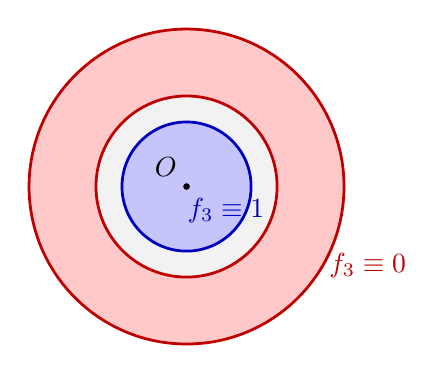
\begin{tikzpicture}[
    inner/.style={
        draw=blue!75!black,
        fill=blue!30,
        fill opacity=0.7,
        draw opacity=1,
        line width=1pt
    },
    outer/.style={
        draw=red!75!black,
        fill=red!30,
        fill opacity=0.7,
        draw opacity=1,
        line width=1pt
    },
    middle/.style={
        draw=red!75!black,
        fill=gray!10,
        line width=1pt
    },
]

% Radii
\def\R{2.0}
\def\r{1.15}

% Outer circle, where outside f_3 = 0
\draw[outer] (0,0) circle (\R);

% Inner circle, boundary of the f_3 = 1 region
\draw[middle] (0,0) circle (\r);

% Green central region
\draw[inner] (0,0) circle (0.82);

\fill[black] (0,0) circle (1.2pt);
\node[above left] at (0,0) {\(O\)};

\node[blue!75!black] at (0.5,-0.3) {$f_3 \equiv 1$};
\node[red!75!black] at (\R+0.3,-1) {$f_3 \equiv 0$};

\end{tikzpicture}
  \]
\end{example}

\begin{definition}[\emph{compactly supported}]
  Let \(M\) be a smooth manifold and \(f:M\to\R\). We define the \emph{support of \(f\)} by \[
    \supp(f) = \overline{\{p \in M : f(p) \neq 0\}}
  \]
  And \(f\) is said to be \emph{compactly supported} if \(\supp(f)\) is compact, we denote the set of all compactly supported smooth functions on \(M\) by \(\mathcal{C}_c^\infty(M)\).
\end{definition}

\begin{lemma}[Existence of Bump Function]\label{lem:bump_exists}
  Let \(M\) be a smooth manifold, \(K\subset M\) be a compact subset and \(U\) be an open neighborhood of \(K\). Then there exists a function \(\f\in C_c^\infty(M)\) such that \begin{enumerate}
    \item \(0 \leq \f \leq 1\),
    \item \(\f \equiv 1\) on \(K\),
    \item \(\supp(\f) \subset U\).
  \end{enumerate}
\end{lemma}
\begin{proof}
  For each \(q\in K\), choose a chart \((\f_q,U_q,V_q)\) centered at \(q\) such that \(U_q\subset U\) and \(B_a(0)\subset V_q\).
  Let \(\wt{U}_q = \f_q^{-1}(B_{a-\eps}(0))\) and \(
    f_q(p) = \begin{cases}
      f_3\circ\f_q(p) & p \in U_q \\
      0 & p \notin U_q
    \end{cases}.
  \)
  \begin{center}
    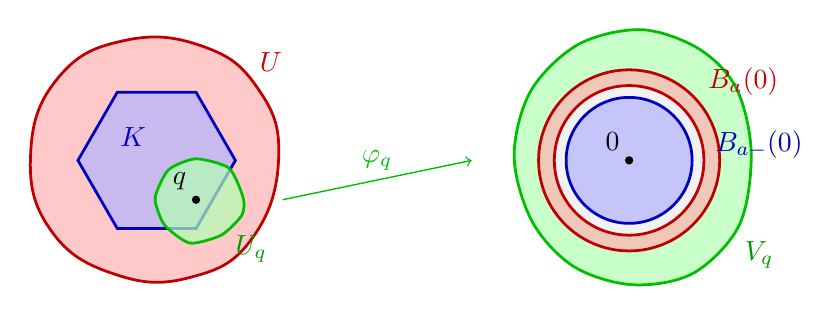
\begin{tikzpicture}[
    bluefill/.style={
        draw=blue!75!black,
        fill=blue!30,
        fill opacity=0.7,
        draw opacity=1,
        line width=1pt
    },
    redfill/.style={
        draw=red!75!black,
        fill=red!30,
        fill opacity=0.7,
        draw opacity=1,
        line width=1pt
    },
    greenfill/.style={
        draw=green!75!black,
        fill=green!30,
        fill opacity=0.7,
        draw opacity=1,
        line width=1pt
    },
    greenarrow/.style={
        ->,
        green!75!black,
        line width=0.5pt
    },
    manifold/.style={
        draw=red!75!black,
        fill=gray!10,
        line width=1pt
    },
    middlearea/.style={
        draw=red!75!black,
        fill=gray!10,
        line width=1pt
    },
  ]
    \def\R{1}
    
    
    % U
    \draw[redfill]
    plot[smooth cycle, tension=0.75] coordinates {
        (1.55,0.05)
        (1.28,0.92)
        (0.58,1.45)
        (-0.42,1.52)
        (-1.25,1.05)
        (-1.60,0.10)
        (-1.35,-0.88)
        (-0.52,-1.45)
        (0.45,-1.48)
        (1.22,-0.98)
    };
    \node[red!80!black] at (1.45,1.25) {\(U\)};

    % K
    \draw[bluefill]
        (0:\R)
        \foreach \angle in {60,120,180,240,300} {
            -- (\angle:\R)
        }
        -- cycle;
    \node[blue!80!black] at (-0.3,0.3) {\(K\)};

    % U_q
    \draw[greenfill]
    plot[smooth cycle, tension=0.40] coordinates {
        (1.10,-0.48)
        (0.92,-0.10)
        (0.50,0.02)
        (0.15,-0.12)
        (-0.02,-0.48)
        (0.10,-0.82)
        (0.42,-1.05)
        (0.82,-0.95)
        (1.08,-0.70)
    };

    \node[green!60!black] at (1.2,-1.12) {\(U_q\)};
    \fill (0.5,-0.5) circle (1.5pt) node[above left] {\(q\)};
    
    % phi_q
    \draw[greenarrow]
      (1.6,-0.5) -- (4,0)
      node[midway,above] {\(\varphi_q\)};
    
    \draw[greenfill]
        plot[smooth cycle, tension=0.55] coordinates {
        (7.55,0.10)
        (7.36,0.92)
        (6.88,1.42)
        (6.15,1.66)
        (5.35,1.47)
        (4.75,0.88)
        (4.54,0.05)
        (4.77,-0.78)
        (5.30,-1.35)
        (6.05,-1.58)
        (6.82,-1.43)
        (7.40,-0.82)
    };
    \node[green!60!black] at (7.65,-1.2) {\(V_q\)};
    
    \draw[redfill] (6,0) circle (1.15);
    \draw[middlearea] (6,0) circle (0.95);
    \draw[bluefill] (6,0) circle (0.8);
    
    \node[red!75!black] at (7.45,1) {\(B_a(0)\)};
    \node[blue!75!black] at (7.65,0.2) {\(B_{a-\eps}(0)\)};
    \fill (6,0) circle (1.5pt) node[above left] {\(0\)};

\end{tikzpicture}
  \end{center}
  We have \(f_q\equiv 1\) on \(\wt{U_q}\) and \(\supp(f_q) \subset U_q\).

  Now we have built an open cover \(\{\wt{U}_q\}_{q\in K}\) of \(K\). We refine it by compactness to \[
    \{\wt{U}_{q_1},\ldots,\wt{U}_{q_N}\} \quad\text{for some } N.
  \]
  Let \(\psi = \sum_{i=1}^N f_{q_i} \in C_c^\infty(M)\), then \(\supp\psi\subset U\) and \(\psi\geq 1\) on \(K\). Finally we put \(\eps = 1\) for \(f_2\) and define \(\f = f_2\circ\psi\). Then for each \(p\in K\) \begin{align*}
    p\in K \implies \psi(p) \geq \eps \implies \f(p) = 1,\\
    p\notin K \implies \psi(p) = 0 \implies \f(p) = 0
  \end{align*} as desired.
\end{proof}

\begin{definition}[\emph{locally finite}]
  Let \(X\) be topological space and \(\{A_\a\}_{\a}\) be a collection of subsets of \(X\). We say that \(\{A_\a\}_{\a}\) is \emph{locally finite} if for each \(p\in M\), there exists an open neighborhood of \(p\) that intersects only finitely many \(A_\a\)'s.
\end{definition}

\begin{definition}[\emph{partition of unity}]
  Let \(M\) be a smooth manifold and \(\{U_\a\}_\a\) be an open cover of \(M\). A \emph{partition of unity subordinate to \(\{U_\a\}_\a\)} is a collection of smooth functions \(\{\f_\a\}_\a\) such that \begin{enumerate}
    \item \(0 \leq \f_\a \leq 1\) for all \(\a\),
    \item \(\supp(\f_\a) \subset U_\a\) for all \(\a\),
    \item \(\{\supp(\f_\a)\}_\a\) is locally finite,
    \item \(\sum_\a \f_\a\equiv 1\).
  \end{enumerate}
\end{definition}

\begin{theorem}[Existence of Partition of Unity]
  Let \(M\) be a smooth manifold and \(\{U_\a\}_\a\) be an open cover of \(M\). Then there exists a partition of unity subordinate to \(\{U_\a\}_\a\).
\end{theorem}
\begin{proof} % TODO
  We will cheat a little and only prove it for compact smooth manifolds \(M\).

  For each \(p\in M\), choose \(\a_p\) such that \(p\in U_{\a_p}\). By putting \(K = \overline{U_{\a_p}}\) into Lemma~\ref{lem:bump_exists},
  we get bump functions \(f_p\in C_c^\infty(U_\a)\) such that \(f_p\equiv 1\) on \(\overline{U_{\a_p}}\).
  By compactness, we can find \(p_1,\ldots,p_N\) such that \[
    M = \bigcup_{i=1}^N U_{\a_{p_i}}.
  \]
  Then \[
    \sum_{i=1}^N f_{p_i} \geq 1 \quad\text{on } M.
  \]
  Finally, construct the partition of unity by \[
    \f_i = \frac{f_{p_i}}{\sum_{j=1}^N f_{p_j}}
  \] as desired.
\end{proof}

The existence of partition of unity leads to \begin{itemize}
  \item Whitney Embedding Theorem,
  \item the definition of integration of differential forms,
  \item the existence of Riemannian metrics.
\end{itemize}

\newpage

\section{Whitney Embedding Theorem}

This section partially follows Guillemin, Pollack: Chapter 1.8.

\begin{theorem}[Weakest version]
  A compact smooth manifold \(M\) can be embedded into \(\R^N\) for sufficiently large \(N\).
\end{theorem}
\begin{proof}
  Left in Homework 2, use partition of unity.
\end{proof}

\begin{theorem}[Median version]
  A compact smooth manifold \(M^m\) can be embedded into \(\R^{2m+1}\).
\end{theorem}
\begin{proof}
  Obtain from the weakest version an embedding \(\Phi:M\to\R^N\) with \(N > 2m+1\).
  We will show that we can project down to \(\R^{N-1}\) and remains an embedding.

  For some \([v]\in\RP^{N-1}\), let \([v]^\perp\) be the orthogonal complement of \([v]\), i.e. \[
    [v]^\perp = \{u\in\R^N\mid \<u,v\> = 0\} \simeq \R^{N-1}.
  \]
  Let \(P_{[v]}:\R^N\to [v]^\perp\) be the linear projection map to the hyperplane \([v]^\perp\), \[
    \begin{tikzcd}
      M \ar{r}{\Phi} &\R^N \ar{r}{P_{[v]}} &\lbrack v\rbrack^\perp \simeq\R^{N-1}.
    \end{tikzcd}
  \]
  We want to show the existence of appropriate \([v]\) such that \(\Phi_{[v]} := P_{[v]}\circ\Phi\) is an embedding.
  \begin{roof}
    It suffices to show the sets \[
      \left\{[v] \mid \Phi_{[v]} \text{ is not injection}\right\}
      \quad\text{and}\quad
      \left\{[v] \mid \Phi_{[v]} \text{ is not an immersion}\right\}
    \] are both measure zero sets in \(\RP^{N-1}\).
    \begin{itemize}
      \item If \(\Phi_{[v]}(p_1) = \Phi_{[v]}(p_2)\), note that \(\ker P_{[v]} = \R v = [v]\), then by linearity, \[
        0 = \Phi_{[v]}(p_1) - \Phi_{[v]}(p_2)
        = P_{[v]}(\Phi(p_1)) - P_{[v]}(\Phi(p_2))
        = P_{[v]}(\Phi(p_1) - \Phi(p_2)),
      \] meaning \([\Phi(p_1) - \Phi(p_2)] = [v]\),
      therefore \([v]\) lies in the image of \begin{align*}
        \a:M\times M &\to\RP^{N-1} \\
        (p_1,p_2) &\mapsto [\Phi(p_1) - \Phi(p_2)].
      \end{align*}
      As \(\dim(M\times M) = 2m < \dim(\RP^{N-1}) = N-1\), \(da_{[v]}\) cannot be surjective, hence \([v]\) is a singular value. It follows Sard's theorem that the set has measure zero.
      \item The other set follows similarly.
    \end{itemize}
  \end{roof}
\end{proof}

This argument does not when when \(N = 2m+1\).
\begin{example}
  If we have \(\Phi:\S^1\to\R^3\) that results in a trefoil knot, then it cannot be projected down to \(\R^2\). This does not contradict the stronger version, since we can simply embed \(\S^1\) into \(\R^2\) by the unknot.
\end{example}

\begin{theorem}[Strong version]
  Any smooth manifold \(M^m\) can be embedded into \(\R^{2m}\).
\end{theorem}
\begin{project}
  Present a complete proof of the Whitney embedding theorem via (finite dimensional) Sard's theorem,
following [Guillemin-Pollack] pp.51--54. For extra credit, do also Exercise 10 on p.55.
\end{project}

This is the best linear bound on the dimension.
\begin{example}
  \(\RP^m\) cannot be smoothly embedded in the space \(\R^{2m-1}\).
\end{example}

There are some even stronger results. 
\begin{proposition}
  Any smooth manifold \(M^m\) where \(m\neq 2^k\), can be embedded into \(\R^{2m-1}\).
\end{proposition}

\begin{proposition}
  Any orientable surface, i.e.\ \(\dim M = 2\), can be embedded into \(\R^3\).
\end{proposition}